\documentclass[sigconf,10pt,nonacm]{acmart}
\settopmatter{printacmref=false, printccs=false, printfolios=true}
\renewcommand\footnotetextcopyrightpermission[1]{}
\pagestyle{plain}
\fancyhead{}
\fancyfoot{}

\usepackage{booktabs}
\usepackage{enumitem}
\usepackage{amsmath,mathtools}
\usepackage{graphicx}
\usepackage{subcaption}
\usepackage{placeins}
\usepackage{microtype}
\usepackage{xspace}
\usepackage{url}

\newcommand{\MI}{mechanistic interpretability\xspace}
\newcommand{\MT}{mechanistic tomography\xspace}
\newcommand{\AtP}{AtP\xspace}
\newcommand{\eps}{\varepsilon}
\newcommand{\R}{\mathbb{R}}
\newcommand{\E}{\mathbb{E}}
\newcommand{\zhat}{\widehat{z}}
\newcommand{\xhat}{\widehat{x}}
\newcommand{\thetahat}{\widehat{\theta}}
\DeclareMathOperator{\logit}{logit}

\newtheorem{theorem}{Theorem}
\newtheorem{lemma}{Lemma}
\newtheorem{proposition}{Proposition}
\newtheorem{corollary}{Corollary}
\newtheorem{observation}{Observation}

\title[Mechanistic Tomography]{Mechanistic Tomography: Designed Measurement for Control-Oriented Interpretability}
\author{Vijay Erramilli}
\email{evijay@gmail.com}

\begin{document}






\begin{abstract}
Mechanistic interpretability seeks quantities that a model does not expose directly: represented states, component effects, interactions, and responses to interventions. Patching, gradients, Hessian-vector products, and subset interventions obtain different measurements under different access assumptions and may target different quantities. We formulate their shared measurement problem as \textbf{mechanistic tomography}: the design and analysis of measurements for recovering internal mechanisms and intervention effects.

For a chosen basis and intervention family, the measurements take the form
\[
\widetilde{y}=Ax+w,
\]
where each row of $A$ describes an intervention, $x$ is the map we want to recover, and $w$ contains nonlinear response, sampling error, and basis misspecification. This gives methods with different targets a common set of questions and a practical sequence: start with the least costly measurements, test on held-out interventions at the intended scale, calibrate a simple mismatch, and expand the family when a structured residual remains. We formalize these decisions through results on measurement error, perturbation design, calibration, and interaction recovery.

The formulation is not specific to control, but control provides a demanding validation setting: once an estimate guides an intervention, it acts as an observer. In a two-HMM belief-state model, control error rises with observer error under a fixed controller and actuator, while target improvement can hide movement of a nuisance state. Under forward-only access, sparse aggregate measurements recover a finite-effect map with fewer interventions than exhaustive coordinate patching. With gradient access, a few finite probes substantially improve a local attribution map, although some held-out gaps remain. Lifted measurements and designed Hessian-vector products recover pair interactions that first-order maps miss, while Tracr shows that the required family depends on the basis. On GPT-2-small IOI, the measurements reproduce conditional backup and identify the Name Mover--Negative Name Mover interaction as the largest held-out predictive term among the three tested cross-group pairs. On Qwen-2.5-7B, a calibrated additive map reaches held-out $R^2=.983$ on a finite refusal-response surface; pairwise lifting gives no detected MAE improvement. The two pretrained-model studies illustrate both branches of the procedure: add interactions when held-out error requires them, and stop at the simpler family when it does not.
\end{abstract}

\maketitle

\section{Introduction}

\begingroup
\emergencystretch=1em
Mechanistic interpretability often asks a simple question: how much does an internal component contribute to a model's output? The model does not report that effect directly, so we have to measure it. Coordinate patching changes one component at a time. Attribution patching uses gradients to estimate many small local effects. Subset interventions change several components together, while Hessian-vector products probe interactions. These methods use different forms of access and may estimate different quantities, but they face the same basic problem: recovering an internal effect from incomplete measurements.
\par
\endgroup

We formulate that problem as $\widetilde y=Ax+w$: each row of $A$ records an intervention, $x$ is the map we want to recover, and $w$ collects what the linear prediction misses. We call the design and analysis of these measurements mechanistic tomography.

Writing the problem this way serves two purposes. The first is structural: it gives methods with different targets a common measurement language. Coordinate patching measures finite one-component effects, attribution patching returns a local gradient map, subset interventions give aggregate forward measurements, and Hessian-vector products measure local curvature~\cite{zhang2024patching,syed2024attrib,bair2026compressed,zhang2026lies}. Their targets remain different. What they share is a set of questions: what is the unknown map, how are the measurements obtained, which interventions do those measurements represent, what does the residual contain, and how will the result be checked? Sec.~\ref{sec:formulation} states this common form and derives the conditions under which its measurements are useful.

The second purpose is operational: the common form shows how an existing method can do more. If an effect map is sparse or compressible, aggregate measurements can replace exhaustive one-component probes. A few finite measurements can test whether a local gradient map needs only a simple correction at the intended intervention scale. If a structured error remains on held-out interventions, the next measurement must add interactions, measure curvature, or change the basis. Calibration dimension names the point at which a simple correction stops being enough; it is one decision inside this larger procedure. Sec.~\ref{sec:decisions} develops this logic. It matters in real transformers because backup, suppression, redundancy, and self-repair make the effect of one component depend on the state of others~\cite{wang2022ioi,mcgrath2023hydra,mcdougall2023copy}.

Current mechanistic interpretability benefits from a strong architectural prior: researchers know where to look because people chose the layers, attention heads, residual streams, and token positions. If models increasingly help design their successors, those conventions may become less transparent to the people evaluating them. This strengthens the case for a measurement-first approach whose claims rest on declared interventions and held-out responses rather than on a familiar blueprint.

We call an estimate an \emph{observer} when it guides an intervention. An observer must do more than reconstruct a mechanism: it must predict what an intervention will actually do at the scale where it will be used---a requirement Sec.~\ref{sec:formulation} develops. Control makes observer error visible: it can change the action taken, and successful target control can still move an unwanted state. Sec.~\ref{sec:control} tests both claims while holding the model, controller, and actuator fixed where required. This use of control follows recent work that evaluates interpretability through the interventions it enables and the evidence supporting them~\cite{bhalla2025unifying,orgad2026actionable}.

The experiments follow the same decision sequence: confirm that observer error reaches a control loop, establish the two first-order branches, then escalate to interactions, the basis, and pretrained models where complete ground truth is no longer available~\cite{lindner2023tracr,wang2022ioi,qwen2025report}. Sec.~\ref{sec:limits} states the boundary of the claim: mechanistic tomography starts after a candidate basis and observer family have been proposed, and it tests those choices rather than discovering the circuit or choosing the controller's objective.

\subsection*{Contributions}

\begin{enumerate}[leftmargin=*,itemsep=2pt]
    \item \textbf{Structural unification.} Table~\ref{tab:methodmap} places coordinate patching, attribution patching, subset recovery, Hessian-vector products, and lifted recovery in one measurement language. The methods keep their own targets and numerical answers; the framework unifies how their measurements and errors are described.
    \item \textbf{Measurement and extension theory.} Lemma~\ref{lem:measurement-reduction} separates nonlinear response, sampling error, and basis error. The remaining results ask when a target can be recovered, how intervention scale and mask density affect the measurements, and when first-order measurements must give way to interaction-aware measurements.
    \item \textbf{Calibration dimension.} Proposition~\ref{prop:caldim} defines the smallest declared correction family that lets a baseline map predict finite responses on held-out interventions. An $r$-dimensional correction needs $O(r)$ well-conditioned probes; a residual outside that family calls for new features or a new basis. Sec.~\ref{sec:step0} tests the dimension-one case: at the larger intervention scale, one fitted gain raises mean held-out AtP $R^2$ from $.818$ to $.960$, close to sparse recovery at $.969$.
    \item \textbf{Control-facing validation.} In a two-HMM wind tunnel, closed-loop target error tracks observer error across ten observer variants (Spearman $0.95$) under a fixed controller and actuator. A separate specificity test shows why target improvement alone is not enough: it can coexist with increased movement of a nuisance state.
    \item \textbf{Operational extensions.} Secs.~\ref{sec:aggregate}--\ref{sec:qwen} follow the procedure under progressively weaker ground truth. Aggregate measurements replace exhaustive coordinate probes when the map is compressible; finite probes calibrate a local gradient map; lifted and curvature measurements recover interactions; Tracr exposes the role of the basis; and GPT-2-small IOI shows when an interaction term is needed. A held-out Qwen-2.5-7B response surface gives the complementary stopping result: finite calibration makes the additive map adequate, so pairwise lifting is not justified by the measured error.
\end{enumerate}

\section{Mechanistic tomography as an inverse problem}\label{sec:formulation}

How much a model's output changes when we alter one or more components\footnote{A component is any unit that can be intervened on; examples include an attention head, MLP block, sparse auto-encoder (SAE) feature, residual-stream direction, or circuit edge.} depends on how we make the measurement. A finite single-component change, a local gradient, and a multi-component intervention need not return the same value because transformers are nonlinear and component effects can depend on what else changes~\cite{zhang2024patching,syed2024attrib,bair2026compressed}. We now make their common measurement structure precise for component-effect maps; Sec.~\ref{sec:control} returns to state estimation for control.

To formalize mechanistic tomography, we first define what we observe, what we change, and over which inputs we average. Let $c\sim\mathcal{D}$ denote a model context, let $h_c$ denote the activation state at the intervention point, and let $f_c(h)$ be the scalar output metric obtained by continuing the model from activation state h under context c. For example, $f_c$ may be a logit difference between two candidate tokens. For each candidate component $i$, the direction $d_i(c)$ specifies how we intervene on that component, and $D_c=[d_1(c),\ldots,d_n(c)]$ represents the set of interventions. These candidate interventions form the coordinate system in which we will estimate component effects. Choosing that coordinate system is an experimental hypothesis; it does not imply that the model’s computation is inherently organized according to those coordinates.

All of these methods begin with the same physical operation. They choose some components, push the activation along their directions, and record how much the readout moves. A method is defined by which components it changes, how far it moves them, and how it turns the measured responses into a map of component effects.

Before comparing these measurements, we need a convention for turning a choice of components into an actual activation change. Without one, a measurement that touches many components may look stronger simply because it changed more of them. Let $z$ be a mask that activates an expected fraction $\rho$ of the coordinates. We choose a normalization $s_\rho>0$ and write $a=z/s_\rho$ for the coefficients applied to the component directions. For example, $s_\rho=\sqrt{\rho n}$ makes the rows of the design approximately unit norm. The scalar $\eps$ sets the overall size of the push. We divide the observed change by $\eps$ so that measurements taken at different scales are reported in the same units:
\begin{equation}
    \widetilde y(a) = \frac{1}{\eps}\E_c\left[f_c(h_c+\eps D_c a)-f_c(h_c)\right].
    \label{eq:finite}
\end{equation}

Each measurement returns one observed number, $\widetilde y(a)$. Up to an error term, that number is a weighted sum of the unknown component effects, and the weights are the entries of $a$. The row $a$ says which components the measurement asked about and how strongly it asked. The unknown map $x$ is what we want to recover. The error term records whatever the weighted sum misses. Methods differ in three ways: how they construct the row, which map they call the target, and what kind of model access produces the measurements.

Coordinate patching puts one nonzero entry in the row. It changes one component at a chosen finite scale and reads that component's finite effect directly. A subset intervention fills several entries at once. No single measurement isolates one component, but several rows together constrain the map. We then solve for the individual effects instead of reading them off one at a time.

Shrinking $\eps$ toward zero changes the target. The finite response becomes a derivative, and the target becomes the local first-order map
\begin{equation}
    x_i = \E_{c\sim\mathcal{D}}\left[\left.\partial_\delta f_c(h_c+\delta d_i(c))\right|_{\delta=0}\right],
    \label{eq:firstorder}
\end{equation}
which attribution patching estimates. This is the degenerate case of the inverse problem assembled below: the backward pass returns the coordinates of $x$ directly, so there is nothing to invert. Coordinate patching at finite $\eps$ uses the same one-coordinate design but returns the finite singleton map instead. For a one-hot row $e_i$, $\widetilde y(e_i)=x_i+w(e_i,\eps)$, so its difference from the local map is exactly the residual we need to measure.

The measurement equation becomes useful for AtP in the forward direction. A gradient supplies $x$ but no information about $w$. An intervention acts at finite scale, where $w$ determines whether $x$ still predicts the response. Measuring that residual requires finite measurements; Sec.~\ref{sec:step0} uses calibration probes for this purpose.

This forward direction is the one an observer exercises. An estimate used to explain a mechanism is checked against that mechanism. An estimate used to guide an intervention must predict the response to an action that has not yet been taken, at the scale the action will use. That second test makes $w$ a first-class quantity and makes $\eps$ and $\rho$ part of the measurement design. Sec.~\ref{sec:control} makes the control loop explicit. The formulation itself does not require a loop, but the intended use determines which residuals matter.

Two further choices stay within the same form. Adding the products $a_i a_j$ to each row adds pair coefficients to the target, so interactions become columns of a larger linear model. A Hessian-vector product along a chosen direction instead measures local curvature. It keeps the same row-times-unknown structure but replaces the effect map with the local curvature map $H_0$.

Stacking $m$ observed responses gives the standard inverse-problem form used in network tomography and compressed sensing~\cite{vardi1996tomo,candes2006robust,firooz2010cs}:
\begin{equation*}
    \widetilde y = A x + w. \tag{MT}
\end{equation*}
Here $\widetilde y$ is the vector of responses we observed, row $j$ of $A$ records the weights used in measurement $j$, and $x$ is the hidden map we want to recover. The residual $w$ collects whatever the weighted sum misses. For a first-order map, this includes curvature, finite-sample error, and error from the chosen basis. One feature differs from a textbook inverse problem: $w$ is not independent noise added to a fixed system. It depends on the design because changing $A$ changes both what we measure and what we do to the model.

This common structure is what mechanistic tomography unifies. The methods all use designed measurements to recover a hidden map, and they face the same questions. Do the measurements contain enough information to recover the map? Is the recovery stable? How many measurements does it cost? What error remains, and does the map work on held-out interventions? The methods need not use the same basis, recover the same map, or require the same model access. A local gradient, a finite singleton effect, and a finite pair effect may therefore have different numerical values.

Why use a linear inverse model rather than a general nonlinear predictor? Once we choose a basis, the simplest useful prediction is a weighted sum with known weights. That form shows whether we have enough independent measurements, whether recovery is stable, whether sparsity can save measurements, and how much the procedure costs. It does not claim that the transformer itself is linear. Anything the weighted sum cannot represent appears in the residual. If that residual remains large on held-out measurements, the experiment must add interactions, change the basis, or use a richer measurement model.

Table~\ref{tab:methodmap} makes this unification concrete by mapping each method to its target, access path, and induced design.

\begin{table}[t]
\centering
\caption{Mechanistic tomography maps each method to a target, access path, and measurement design.}
\label{tab:methodmap}
\scriptsize
\renewcommand{\arraystretch}{1.08}
\setlength{\tabcolsep}{2pt}
\begin{tabular}{p{0.27\linewidth}p{0.28\linewidth}p{0.35\linewidth}}
\toprule
Method and access & Declared target & Induced measurement \\
\midrule
Coordinate patching; forward & finite singleton effects & one-coordinate rows \\
Subset recovery; forward & additive finite map & multi-coordinate rows; joint fit \\
AtP; backward & local first-order map $x$ & gradient returns coordinates \\
Lifted recovery; forward & finite main and pair effects & columns include $a_i$ and $a_i a_j$ \\
HVP; white-box second order & local curvature $H_0$ & directions give curvature projections \\
\bottomrule
\end{tabular}
\end{table}
\FloatBarrier

\subsection{What the formulation lets us decide}\label{sec:decisions}

The inverse formulation separates three decisions that arise in any measurement-based study of mechanism. First, does the proposed linear relation describe finite interventions at the scale where the estimate will be used? Second, if it does, which measurement design identifies the target with acceptable cost and error? Third, if the relation fails on held-out interventions, can a small calibration repair it, or must the measurement family be enlarged? These are the natural questions because they are the three stages of an inverse measurement procedure: model the measurements, recover the target, and diagnose the model when it fails.

This is a design principle, not a reporting preference. A map should be tested in the operating region where it will be used, rather than only where it is easiest to measure. For an observer, that region is set by the intervention scale and the contexts the controller will encounter. Held-out finite interventions therefore test whether the map is adequate for action.

Two criteria are in play, and they will often agree. One asks whether the estimate faithfully recovers the declared target; the other asks whether it supports the intended action. They can come apart because a downstream use weights errors unevenly. Error in directions the actuator cannot express may have little effect on the loop, while error along its effective direction matters directly. Reconstruction accuracy remains the right criterion for explanation. When an estimate will drive an intervention, reconstruction and control performance should be reported separately. Sec.~\ref{sec:result-control} gives a case in which they diverge. The same distinction appears in network tomography~\cite{roughan2003te}.

The recovery tools come from classical inverse problems, sparse recovery, masked interaction recovery, and HVP correction~\cite{bair2026compressed,kang2025spex,butler2025proxyspex,zhang2026lies}. The new element is that each measurement is also a finite intervention on a nonlinear model, so the design changes the residual it must control.

\paragraph{Does one finite intervention produce a linear measurement?}
The inverse formulation would be empty if we simply assumed that every intervention followed it. We instead derive the relation from the response to one finite intervention. The lemma below shows that a mask $a$ produces a weighted sum of the local component effects, $a^\top x$, plus three identifiable sources of error.

\begin{lemma}[Mechanistic measurement reduction]\label{lem:measurement-reduction}
Let $f_c$ be twice differentiable on the perturbation ball. Assume its Hessian satisfies $\|\nabla^2 f_c\|_{op}\le L$. Define the population normalized response
\begin{equation}
    y_\infty(a,\eps)
    =
    \frac{1}{\eps}
    \E_c\!\left[
    f_c(h_c+\eps D_ca)-f_c(h_c)
    \right].
\end{equation}
Suppose the response estimated from a batch of $B$ paired contexts can be written as
\begin{equation}
    \widetilde y_B(a,\eps)
    =
    y_\infty(a,\eps)
    +\frac{e_B(a)}{\eps}
    +\zeta_B(a,\eps),
\end{equation}
where $|e_B(a)|\le\tau_B(a)$ bounds uncancelled error in the response numerator and $|\zeta_B(a,\eps)|\le\nu_B(a)$ bounds the remaining normalized sampling error. Then
\begin{equation}
    \widetilde y_B(a,\eps)
    =
    a^\top x+w(a,\eps),
\end{equation}
where $x$ is the local first-order map in Equation~\eqref{eq:firstorder} and
\begin{equation}
    |w(a,\eps)| \le \frac{L}{2}\eps\E_c\|D_ca\|_2^2
    + \frac{\tau_B(a)}{\eps}+\nu_B(a).
\end{equation}
Stacking measurements from several masks gives $\widetilde y=Ax+w$. The proof is in Appendix~\ref{app:proof-measurement}.
\end{lemma}

A simple example makes the result concrete. Suppose a mask changes only heads 2 and 5, with coefficients $a_2$ and $a_5$. The linear part of the measured response is
\[
    a^\top x=a_2x_2+a_5x_5.
\]
The intervention does not reveal either effect separately. It returns one weighted sum of them. Several masks produce several such equations, and solving those equations recovers the individual effects. This is the same logic used in network tomography and compressed sensing.

The residual $w$ records why the measured transformer response may differ from that weighted sum. Its three terms describe three different problems. The curvature term grows with $\eps$: a larger intervention moves farther from the local tangent and encounters more of the model's nonlinear response. The term $\tau_B/\eps$ grows when $\eps$ becomes too small: any error already present in the response numerator is magnified when we divide by the intervention size. The remaining term $\nu_B$ records normalized sampling error that remains after pairing or batching.

The lemma therefore rules out both extremes. We cannot make the intervention arbitrarily large, because curvature then dominates. We cannot make it arbitrarily small when numerator error remains, because normalization magnifies that error. Pairing the clean and intervened evaluations helps because it can cancel shared variation before division by $\eps$.

The mask affects more than the row of $A$. It also changes the displacement $\|D_ca\|$, the amount of curvature encountered, and potentially the sampling error. The design matrix and the residual are therefore coupled. This is the main difference from a textbook linear inverse problem with independent noise added after the measurements have been chosen.

The lemma establishes a local measurement model. It does not yet say that $A$ contains enough information to recover $x$, that $x$ is sparse, or that the residual is independent noise. Those are separate questions. The next results ask whether the design identifies the target, how scale and density affect its error, and when a persistent residual requires calibration or a richer feature family.

\paragraph{Can a small correction repair the finite response?}
For a nondifferentiable endpoint---for example, a behavioral rating, tool outcome, or black-box score---we cannot use the Taylor bound directly. In that setting the finite response is the quantity of interest, and held-out interventions provide the relevant test. The remaining question is whether the difference from the gradient map is a simple scale correction or evidence that the first-order family is missing structure. Calibration dimension formalizes that distinction.

A useful first check is whether all finite effects are approximately a rescaled version of the local map. If so, a few finite probes may be enough to estimate the correction. If not, collecting more probes for the same family will not solve the problem.

\begin{proposition}[Calibration dimension]\label{prop:caldim}
Let $F_\eps(a)$ denote the systematic finite-intervention response on a design family $\mathcal A$, and let $\mathcal Q$ be a declared held-out distribution on that family. Fix a declared feature map $\phi(a)\in\R^q$, baseline $x_0\in\R^q$, and correction dictionary $B\in\R^{q\times r}$. If
\begin{equation}
    F_\eps(a)=\phi(a)^\top(x_0+B\theta_\eps)
    \quad\text{for all } a\in\mathcal A
\end{equation}
and the sampled correction design $\Phi B$ has full column rank, then $\theta_\eps$ is identifiable from $O(r)$ noiseless calibration measurements and stably estimable according to the conditioning of $\Phi B$, where row $j$ of $\Phi$ is $\phi(a_j)^\top$. If no such $\theta$ exists, the residual
\begin{equation}
    \inf_\theta \|F_\eps(\cdot)-\phi(\cdot)^\top(x_0+B\theta)\|_{L_2(\mathcal Q)}
\end{equation}
lower-bounds the error of every observer using that family.
\end{proposition}

For a declared nested family $B_r$ and a tolerance $\delta$ at or above the estimated noise floor, the calibration dimension is the smallest $r$ whose held-out error is at most $\delta$. Dimension zero means that the baseline map transfers without correction. Dimension one allows one scalar gain. Larger values allow several stated corrections, such as separate gains for component groups. If the residual lies outside the entire first-order family, no collection of gains can fix it; the observer needs new features, such as component pairs. Sec.~\ref{sec:step0} tests the one-gain case; Sec.~\ref{sec:interactions} supplies a case in which pair features are necessary.

Appendix~\ref{app:calibration} gives concrete examples of what low and high calibration dimension mean.

This definition gives a practical stopping rule. Start with a gradient map when a backward pass is available; otherwise start with an additive map estimated from forward interventions. Fit the correction on one set of masks and evaluate it on another. The held-out split matters because curvature and correlated masks can make an inadequate family fit its training measurements. In the ideal noiseless case, an $r$-dimensional correction needs only $O(r)$ well-conditioned probes instead of re-estimating $n$ main effects or $O(n^2)$ pairs. Move to a richer family only when the held-out residual remains above the estimated noise floor and the richer family improves it reproducibly.

\paragraph{How should scale and mask density be chosen?}
After choosing an observer family, we still need to choose the interventions used to measure it. Two design variables matter immediately. The scale $\eps$ controls how far each probe moves the model, while the density $\rho$ controls how many coordinates each mask changes. Small probes reduce nonlinear error but magnify uncancelled response noise. Dense masks may cover sparse features more efficiently, but they can also move the activation farther or make the inverse problem poorly conditioned.

\begin{corollary}[Noisy first-order scale--density bound]\label{cor:scale-density}
For a mask family $\mathcal A_\rho$ under a fixed actuator normalization, define
\begin{equation}
    \kappa_\rho^2 = \sup_{a\in\mathcal A_\rho}\E_c\|D_ca\|_2^2,
\end{equation}
and let $\tau_B(\rho)$ and $\nu_B(\rho)$ uniformly bound the two sampling terms in Lemma~\ref{lem:measurement-reduction}. If $C_{\mathrm{rec}}(A_\rho)$ bounds the selected recovery method's amplification of measurement error, a conditional first-order error objective is
\begin{equation}
\begin{aligned}
    \mathcal J_1(\eps,\rho)
    &= C_{\mathrm{rec}}(A_\rho)
    \left[
    \frac{L}{2}\eps\kappa_\rho^2
    +\frac{\tau_B(\rho)}{\eps}+\nu_B(\rho)
    \right],\\
    (\eps^*,\rho^*)&\in\arg\min_{\eps,\rho}\mathcal J_1(\eps,\rho).
\end{aligned}
\end{equation}
For fixed $\rho$, if $\tau_B(\rho)>0$ and $C_{\mathrm{rec}},\nu_B$ are locally independent of $\eps$, the first two terms are minimized at
\begin{equation}
    \eps^*(\rho)=\sqrt{\frac{2\tau_B(\rho)}{L\kappa_\rho^2}}.
\end{equation}
Density affects both model-induced error through $\kappa_\rho$ and identifiability through coverage and conditioning.
\end{corollary}

The bound guides what a scale--density study must measure; it is not a post-hoc derivation of the settings used here. Secs.~\ref{sec:aggregate}--\ref{sec:interactions} vary scale, budget, and noise separately rather than estimating $L$, $\tau_B$, or the full $\eps\times\rho$ surface. Sec.~\ref{sec:discussion} returns to this limitation.

Appendix~\ref{app:scale-density} unpacks the scale and density terms in plain measurement-design language.

\paragraph{What the bound shows.}
The square-root dependence of the preferred scale comes from classical noisy forward differences~\cite{shi2022finite}. Mechanistic interventions add two complications. First, the mask family changes the activation displacement as well as the coverage of the unknown components. Second, the same family changes the conditioning of the recovery problem. The term $\tau_B$ represents response error that is present before division by $\eps$ and does not cancel between the clean and intervened evaluations; $\nu_B$ represents the paired sampling error left after normalization. Mask density has no meaning without an actuator convention. Under fixed per-coordinate amplitude, a denser mask usually causes a larger displacement. Under unit-row normalization, it need not. For pair or Hessian targets, some quadratic response becomes signal rather than error, but mask density still controls whether the pair features receive enough independent coverage.

\paragraph{Sparse-recovery consequences.}
If the component-effect map is sparse or compressible, aggregate masks can recover it with fewer forward evaluations than patching every coordinate. Once the measurement relation holds, basis pursuit and orthogonal matching pursuit (OMP) use the standard sparse-recovery guarantees, provided that the mask design is sufficiently well conditioned~\cite{candes2006robust,tropp2007omp,berinde2008expander}. Coordinate-only forward patching has a simple worst-case limitation: with fewer than $n$ measurements, at least one coordinate remains unmeasured, and the entire effect may be hidden there. This is a minimax statement, not a claim about average model behavior. It also applies only to forward-only recovery; a white-box gradient returns all first-order coordinates in one backward pass.

\paragraph{Why first-order maps miss interactions.}
Sparse recovery cannot recover a term that the measurement model does not contain. This matters for real transformers. Softmax attention, layer normalization, nonlinear MLPs, and downstream heads all allow the effect of one component to depend on the state of another. Backup heads may compensate for an ablated primary head; self-repair can reroute a computation; and copy-suppression heads act conditionally on what earlier heads have written~\cite{wang2022ioi,mcgrath2023hydra,mcdougall2023copy}. An additive model cannot express these dependencies. More first-order measurements only estimate the wrong family more accurately. Pair features are the smallest extension that can represent a two-component interaction.

\begin{proposition}[First-order blindness to pure interactions]\label{prop:blindness}
Let $H_{0,ij}=\partial^2 f/\partial d_i\partial d_j$ at the baseline. If $x_i=x_j=0$ but $H_{0,ij}\ne0$, gradients and singleton first-order measurements do not identify the cross term. At scale $\eps$, the normalized finite response has
\begin{equation}
    \widetilde y(a)=a^\top x+\sum_{i<j}a_i a_j\Gamma_{\eps,ij}+w_\eps(a),
\end{equation}
where $\Gamma_{\eps,ij}=\eps H_{0,ij}+O(\eps^2)$. Lifted features $a_i a_j$ make these finite pair coefficients visible.
\end{proposition}

The lifted model treats each product $a_i a_j$ as an additional measurement feature. It can make a pair visible, but it also creates many more columns: $n$ main effects become $n+\binom{n}{2}$ main-and-pair effects. A design that is well conditioned for the original $n$ columns may be badly conditioned after this expansion.

\begin{proposition}[Conditional lifted-recovery reduction]\label{prop:lifted}
Let $\theta_\eps=(x_\eps,\mathrm{vec}\,\Gamma_\eps)\in\R^{N}$ be sparse in a lifted finite main-plus-pair basis, and let $\Phi(A)$ be the corresponding lifted design with rows $[a,\{a_i a_j\}_{i<j}]$. If the lifted misspecification is bounded, sparse recovery gives the same form of stable error bound as classical sparse recovery, conditional on restricted conditioning of $\Phi(A)$ on the relevant support. A first-order restricted-isometry property (RIP) does not imply lifted RIP. Appendix~\ref{app:proof-lifted} gives the reduction to the standard sparse-recovery theorem.
\end{proposition}

With ideal dense independent Rademacher masks, whose entries are independent random $+1$ or $-1$ values, the main-effect columns $a_i$ and pair columns $a_i a_j$ are orthogonal in the population. Real designs are finite and often sparse or constrained. Pair columns can then duplicate or nearly duplicate one another. We must therefore inspect the conditioning of the lifted design and test the recovered map on masks that were not used for fitting.

Appendix~\ref{app:lifted-conditioning} gives a two-component example of this aliasing problem.

Held-out prediction is therefore part of identification, not merely a reporting convention. On the training masks, a true pair and a false pair can produce the same column and appear equally plausible. A separate or deliberately de-aliased mask design tests whether the recovered interaction transfers.

\paragraph{How should missing interactions be measured?}
White-box access solves the first-order part cheaply, but one backward pass still does not return the full pair map. We need measurements of curvature as well. A Hessian-vector product (HVP) measures how the gradient changes along a chosen direction without constructing the full Hessian, so designed HVP directions can serve as aggregate measurements of local interactions.

\begin{corollary}[White-box second-order tomography]\label{cor:hvp}
A backward pass gives $\nabla f$, while designed HVP queries give linear measurements of the local curvature map $H_0$. If the response is quadratic on the intervention path, the known relation $\Gamma_\eps=\eps H_0$ converts local curvature to the normalized finite pair map. Otherwise HVPs identify only a local quantity; finite-scale prediction needs path integration or finite calibration. Lifted forward measurements estimate the finite-scale map directly. Integrated Hessians and HVP correction provide precedents~\cite{janizek2020integrated,zhang2026lies}.
\end{corollary}

The access regime again determines the efficient route. With gradients and HVPs, we can estimate local main and pair effects without evaluating every finite mask. With only forward evaluations or with a nondifferentiable endpoint, lifted subset interventions measure the finite pair response directly. The two routes target the same quantity only when local curvature transfers to the finite intervention scale; otherwise we must integrate along the path or calibrate against finite responses.

Appendix~\ref{app:remaining-proofs} gives the proofs of the calibration, scale--density, interaction-blindness, and HVP results.

\section{What the formulation cannot decide}\label{sec:limits}

The inverse formulation isolates a recovery step for which standard tools are available. It does not, however, choose the objects that give that recovery meaning. The researcher must choose the basis that defines the coordinates of $A$ and $x$, state what $x$ is meant to estimate, and declare the context distribution over which the measurements are averaged and expected to transfer. The model supplies none of these choices. This section states them explicitly; the experiments then place each one under control.

\paragraph{The basis is not given.}
Layers, attention heads, MLPs, residual subspaces, SAE features, and token positions are all plausible coordinates. They make different claims about the units of the mechanism. A mechanism that is sparse in one basis can look distributed in another. A poorly chosen coordinate can also track the output without playing the proposed causal role. Basis selection is therefore closer to dictionary learning than to regression with known features~\cite{arora2014dictionary}. Superposition and the non-uniqueness of SAE dictionaries make the choice substantive rather than cosmetic~\cite{elhage2022superposition,leask2025canonical}. Secs.~\ref{sec:interactions} and~\ref{sec:basis} put this choice under control: the planted harness fixes the basis by construction, while Tracr lets us vary the basis without losing knowledge of the computation.

\paragraph{Behavioral success does not establish the target.}
A direction can change behavior without representing the variable we think it represents. For example, an entropy-aligned direction may predict uncertainty and provide a useful steering axis even if it is not the model's belief state or a causal bottleneck~\cite{agarwal2025scaling}. Successful control therefore does not identify the mechanism by itself. We need an independent reference, such as an analytic posterior, a planted or compiled circuit, or a causal intervention test~\cite{agarwal2025geometry,geiger2024das,geiger2025causal}. Sec.~\ref{sec:result-control} supplies such a reference and asks what happens when observer error reaches a control loop.

\paragraph{The target depends on the context distribution.}
Equation~\eqref{eq:firstorder} averages effects over a declared context distribution. If the local response changes direction across prompts, one average can mix distinct mechanisms and describe none of them well. A component-effect map is therefore tied to the contexts used to construct it. The held-out evaluation must preserve the variation expected when the observer is used. Sec.~\ref{sec:ioi} returns to this issue in a pretrained model, where the ranking of interaction terms is stated for a specific intervention and prompt distribution.

The experiments place these three objects under control and then relax that control one step at a time. The HMM supplies an exact reference for the target quantity. The planted harness fixes both the basis and the nonzero support. Tracr keeps the computation known while the basis changes. IOI retains documented component groups and a declared intervention distribution, but no complete mechanism ground truth. Each step gives up one kind of external reference only after the preceding measurement question has been checked.

\section{Control-facing validation}\label{sec:control}

Before testing the operational extensions, we run two control checks. First, we hold the transformer, actuator, and controller fixed and vary only the observer, which isolates whether observer error reaches the control loop. Second, a target--nuisance estimate drives a correspondingly mixed actuation direction, which asks whether target improvement can hide nuisance movement. Here an \emph{observer} is any estimate that guides an intervention.

A control-oriented description separates four objects that steering experiments often merge. The transformer has an internal activation state $x_t$; in classical control terminology, it is the \emph{plant}.\footnote{More precisely, the controlled system includes the transformer state at the edit location and the remaining computation from that state to the readout. We use \emph{transformer} in the text and reserve \emph{plant} for this classical control-theory meaning.} The quantity we want to regulate is $z_t=\phi(x_t)$, but the controller does not observe it directly. It receives measurements $y_t$, uses an observer $O$ to form the estimate $\widehat z_t$, and then applies a control rule $K$:
\begin{align}
    z_t &= \phi(x_t), & y_t &= h(x_t,c_t)+\epsilon_t,\\
    \zhat_t &= O(y_{0:t},c_{0:t}), & u_t &= K(\zhat_t,r_t).
\end{align}
Here $c_t$ denotes the context, $\epsilon_t$ measurement noise, $r_t$ the desired reference, and $u_t$ the intervention. In an activation-steering example, $x_t$ is the residual-stream state, $O$ is a probe or another state estimate, $K$ converts the estimated error into an edit size, and the actuator is the direction along which the activation is changed. The intervention could instead be a logit bias, retrieval insertion, prompt rewrite, or decoding change. Even a well-behaved controller $K$ can fail if the observer $O$ estimates the wrong quantity. We therefore validate the estimate in four ways: agreement with an oracle when one exists, sensitivity under a fixed controller, movement of nuisance variables, and prediction on held-out interventions in a real model.

\begin{figure}[t]
\centering
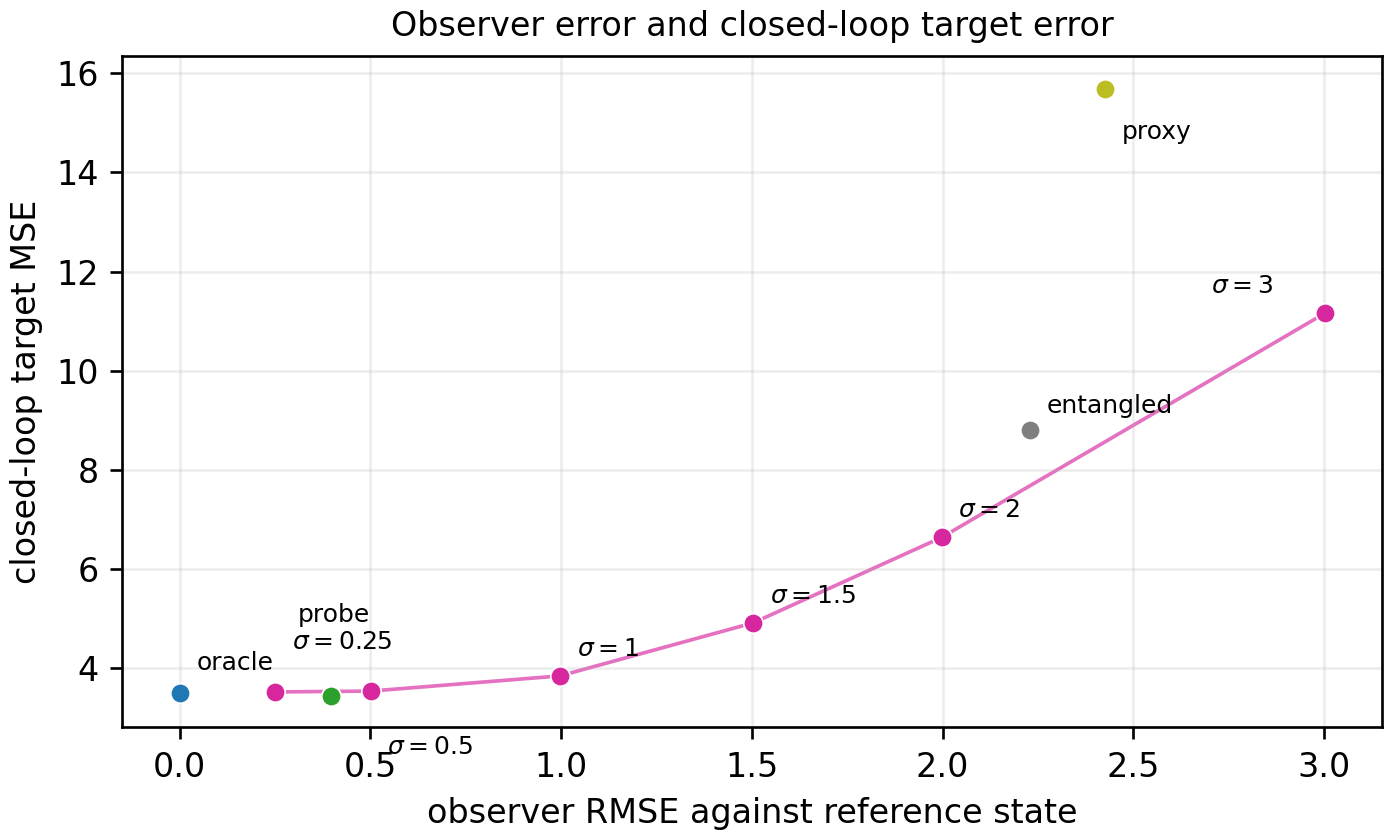
\includegraphics[width=0.82\linewidth]{figs/observer_control.png}
\caption{With the controller and actuator fixed, closed-loop target error rises with observer error across ten observer variants. Oracle and probe lie low-left; coarse, noisy, proxy, and entangled estimates move up and right.}
\label{fig:observer}
\end{figure}

\subsection{Observer error reaches the loop; target success can hide nuisance movement}\label{sec:result-control}
We need a setting in which the quantity an observer should recover is known exactly. A hidden Markov model (HMM) supplies that reference: after every token, we can compute the exact filtered posterior over its changing hidden state. We can therefore measure observer error before placing the estimate in a feedback loop. This is the reason for starting with an HMM rather than a natural-language task, where the model's true internal belief is not available.

Building on analytic-posterior HMM wind tunnels~\cite{agarwal2025geometry}, we train a small transformer on tokens generated by two independent HMMs. One hidden process defines the target belief $z_1$; the other defines a nuisance belief $z_2$. We use their exact posterior log-odds as the two reference states. The model reaches the Bayes cross-entropy floor, and a linear probe recovers $z_1$ with $R^2\approx0.99$.

The first check asks whether observer quality matters once the estimate enters a feedback loop. We create ten observers with different amounts and kinds of error, including a last-observation proxy that uses only the current emission instead of the filtered history. We then hold the transformer, actuator, controller, and target fixed. Across these observers, closed-loop target error rises with observer RMSE (Spearman $r_s=0.95$). This is a necessary sanity check for the rest of the paper: if observer error did not affect control in a known-state setting, better measurement would have no demonstrated downstream value.

The second check asks a different question. Can an observer improve the target while moving an unrelated state? We deliberately mix the target and nuisance estimates as $z_1+0.5z_2$ and use the corresponding mixed actuation direction $d\propto d_1+0.5d_2$. This condition reduces target MSE from $25.02$ without control to $4.81$, while the oracle target-only condition reaches $3.56$. Yet nuisance movement rises from $0.037$ to $0.079$. Because this stress test changes both the observer and the actuator, it does not isolate observer error. It establishes the narrower point for which it was designed: target improvement alone does not show that the control action used the intended internal direction.

The two criteria mostly agree here, and where they do not, the reason is instructive. The linear probe sometimes produces slightly lower closed-loop error than the analytic posterior oracle, even though the oracle is the more faithful estimate of the external HMM posterior. The controller edits the state represented by the transformer, and the probe can align more closely with that editable state than the external posterior does. This is a measured separation between reconstruction and control utility. We therefore report both: the analytic posterior tests representational faithfulness, while closed-loop performance tests how well an observer matches the state used by this model--actuator pair.

Having shown that observer error reaches the control loop and that target gains can mask collateral movement, we can ask the operational question: how cheaply can an adequate observer be measured under each access regime? We keep the model and task fixed and begin with first-order measurements under forward-only and white-box access.

\section{Operational extensions}\label{sec:extensions}

The experiments below test the operational extensions developed in Sec.~\ref{sec:decisions}, beginning with forward-only access.

\subsection{Aggregate measurements replace exhaustive probes when the map is compressible}\label{sec:aggregate}

Without gradient access, coordinate patching requires a separate forward intervention for every coordinate. Mechanistic tomography suggests another option: change several coordinates together and treat the response as one aggregate measurement. Each such intervention supplies one row of $A$. If only a few coordinates have large effects, several aggregate rows may recover the map with fewer interventions than probing every coordinate separately.

We test this possibility in the same HMM model used for the control experiment. We define 32 coordinates by crossing transformer layer with token position. This dimension is small enough that we can also patch all 32 coordinates individually. Their finite effects provide a reference against which to evaluate the aggregate recovery.

The reference map is not exactly sparse, but it is strongly compressible: its four largest coordinates contain $98.4\%$ of its squared $\ell_2$ norm. We therefore use orthogonal matching pursuit (OMP), a sparse-recovery method that selects a small set of coordinates and fits their effects from the aggregate responses. A separate validation split chooses how many coordinates OMP should retain. We also fit ridge regression as a dense baseline.

After 12 aggregate measurements, validation selects a four-coordinate OMP model. It reaches Pearson $r=0.989$ against the coordinate-patching reference and $R^2=0.935$ on held-out aggregate masks. Ridge regression requires 32 measurements, the same count as exhaustive coordinate patching, to reach $r=0.962$ and held-out $R^2=0.933$.

This is a positive but conditional result. Aggregate measurements save interventions here because the finite-effect map is compressible and the aggregate response is approximately additive. They would not provide the same advantage for a dense map or one dominated by interactions. Bair et al. demonstrate the same sparse-recovery principle at pretrained-model scale using attention-head knockouts~\cite{bair2026compressed}. Here the experiment establishes the forward-only baseline before we consider the cheaper access provided by gradients.

\begin{figure}[t]
\centering

\includegraphics[width=0.82\linewidth]{figs/nt_sample_efficiency.png}
\caption{Aggregate recovery of the 32-coordinate finite-effect map. OMP scores Pearson $r=0.989$ and held-out $R^2=0.935$ with 12 aggregate measurements. Ridge reaches comparable held-out prediction with 32 measurements, the exhaustive coordinate count.}
\label{fig:forward}
\end{figure}

\subsection{A few finite probes calibrate attribution patching at intervention scale}\label{sec:step0}

With gradient access, attribution patching returns the complete local first-order map in one backward pass. This is cheaper than recovering the same map from many forward measurements. The limitation is that a gradient describes an infinitesimal change, while an actual intervention has finite size. Curvature and saturation can make the finite response smaller than, or otherwise different from, the gradient prediction.

We therefore ask the cheapest question first: is the mismatch mostly a single scale factor, or is the local map missing structure? We test two intervention scales, $\eps\in\{5,8\}$, using the same trained HMM model and component directions as in Sec.~\ref{sec:aggregate}. Raw AtP already predicts the smaller intervention well. At $\eps=8$, saturation makes the finite response smaller than the gradient extrapolation, so raw AtP systematically overpredicts it. We fit one scalar gain from a set of finite calibration probes and apply it to the entire gradient map. This correction changes the scale of the map without re-estimating its coordinates.

A gain can look successful simply because it was fitted on a favorable set of sequences or masks. We therefore cross three independently generated evaluation batches with three independently generated mask-and-split designs, giving nine evaluation cells. Each cell contains 128 masks. We use 72 to fit the scalar gain and the sparse OMP comparison, 24 to select the OMP model, and 32 only for final evaluation. The gain may depend on intervention scale; we do not treat it as a universal property of the model.

\begin{table}[t]
\centering
\caption{Finite-scale calibration on one trained model whose intervention directions are estimated once. We cross three independently generated 256-sequence evaluation batches with three mask-and-split designs. Entries are means [min, max] across the nine cells.}
\label{tab:step0}
\scriptsize
\setlength{\tabcolsep}{3pt}
\begin{tabular}{lrrrr}
\toprule
Scale & raw AtP $R^2$ & calibrated AtP $R^2$ & OMP $R^2$ & fitted gain $\widehat g$ \\
\midrule
$\eps=5$ & 0.943 [0.920, 0.967] & 0.963 [0.933, 0.983] & 0.965 [0.952, 0.976] & 0.874 [0.799, 0.915] \\
$\eps=8$ & 0.818 [0.751, 0.903] & 0.960 [0.925, 0.978] & 0.969 [0.960, 0.977] & 0.742 [0.677, 0.780] \\
\bottomrule
\end{tabular}
\end{table}

At $\eps=8$, calibration raises mean held-out $R^2$ from $0.818$ to $0.960$, close to OMP's $0.969$. A gain fitted on the other two evaluation batches gives a leave-one-batch-out mean of $0.959$ across the nine target/design cells. The correction therefore transfers across sequence batches rather than merely fitting one set of examples. At $\eps=5$, where raw AtP is already strong, calibration raises mean held-out $R^2$ from $0.943$ to $0.963$, compared with $0.965$ for OMP.

We next ask how many finite probes the correction needs. From the 96 masks not reserved for final evaluation, we repeatedly draw calibration sets of 4, 8, and 16 probes; the 96-probe condition uses the full pool. Eight probes already give mean held-out $R^2=0.951$ at $\eps=5$ and $0.948$ at $\eps=8$. Sixteen probes raise these values to $0.957$ and $0.955$. This is why calibration is the first extension to try when gradients are available: a handful of finite measurements can correct most of the scale error without recovering the component map again.

The result is positive, but it is not a blanket endorsement of scalar calibration. A scalar correction is the calibration-dimension-one hypothesis. Even after all 96 probes, some evaluation-batch/design cells retain a gap to OMP. The data therefore support the scalar gain as a useful approximation, not as an exact description of the finite map. Held-out error supplies the stopping rule: stop when the corrected map predicts the intended interventions well enough; otherwise move to a richer observer.

\begin{figure}[t]
\centering
\begin{subfigure}{0.49\linewidth}
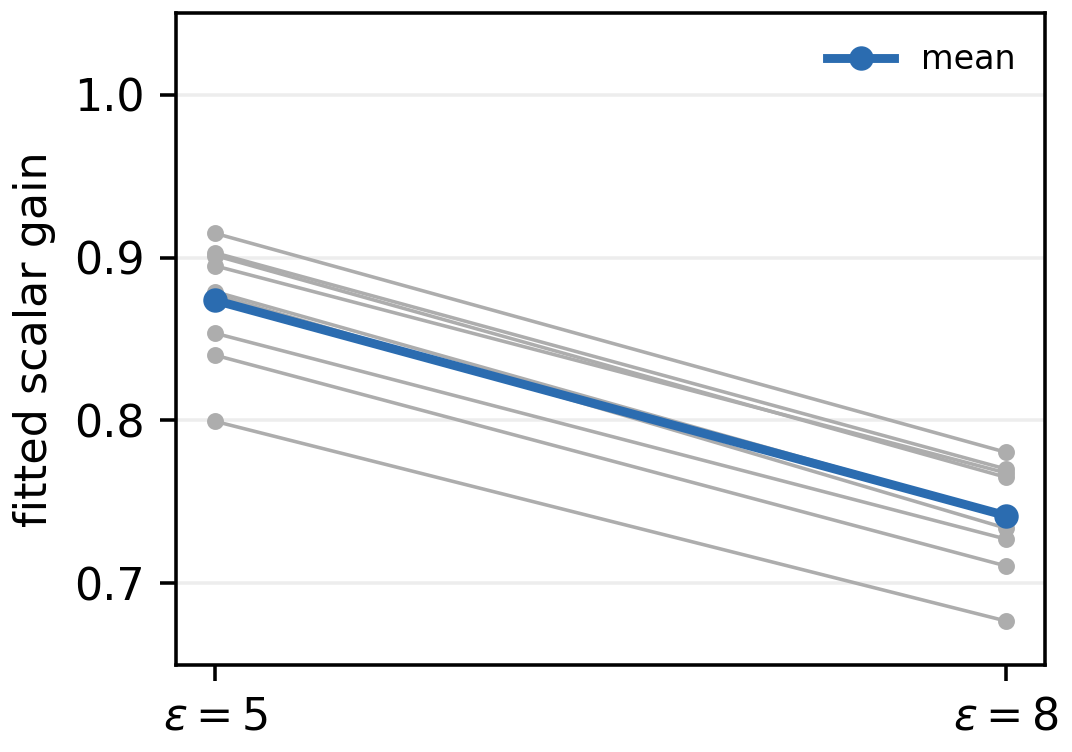
\includegraphics[width=\linewidth]{figs/calibration_factorial_gain_pairs.png}
\caption{Gain shift with scale}
\end{subfigure}\hfill
\begin{subfigure}{0.49\linewidth}
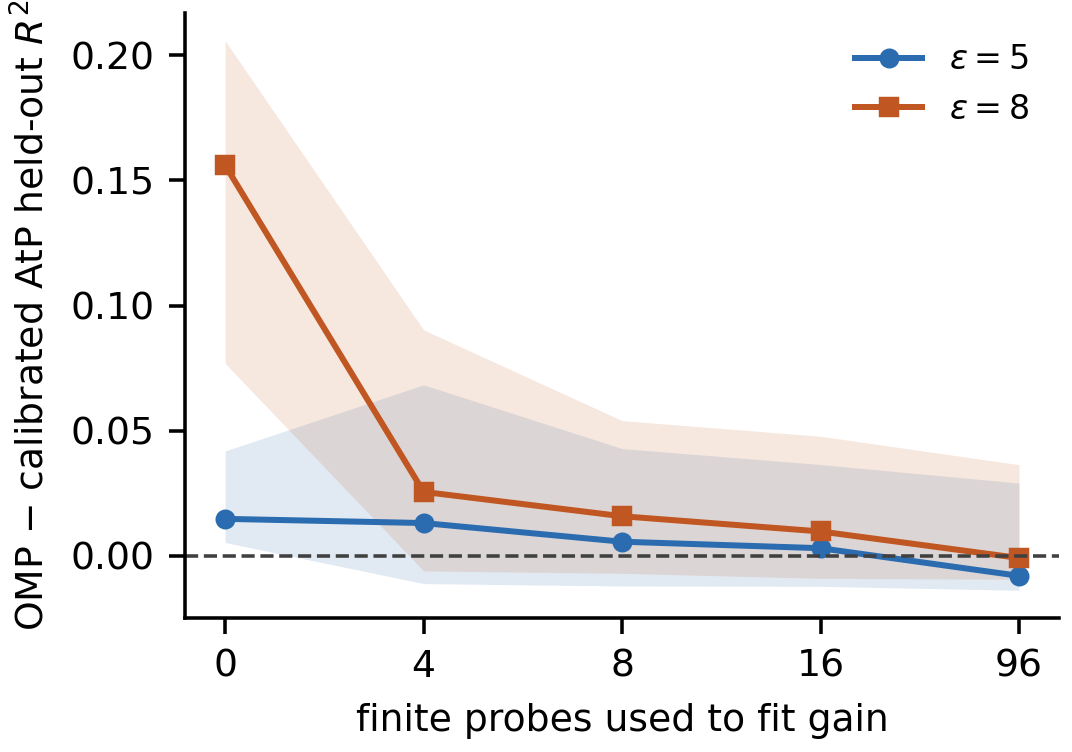
\includegraphics[width=\linewidth]{figs/calibration_factorial_gap_to_omp.png}
\caption{Small-budget calibration}
\end{subfigure}
\caption{Finite-scale calibration across the fixed-direction $3\times3$ design. Left: fitted gain at each scale for the nine evaluation-batch/design cells. Right: the median held-out $R^2$ gap between OMP and calibrated AtP as the calibration budget grows; bands show the 10th--90th percentiles over cells and subset draws.}
\label{fig:step0}
\end{figure}

\FloatBarrier
\subsection{Interaction measurements recover effects that first-order maps miss}\label{sec:interactions}

Scalar calibration can change the size of a first-order effect, but it cannot create an effect that appears only when two components change together. If the response contains a term such as $a_i a_j$, no gain applied to an additive map can represent it. This matters for transformers because backup, suppression, redundancy, and self-repair make the effect of one component depend on whether another is active. Before studying these effects in a pretrained model, we use a planted system in which the correct terms are known. This lets us distinguish three failures that can otherwise look alike: choosing a family that cannot represent the response, collecting too few measurements, and selecting a correlated but noncausal feature.

The harness contains 64 candidate components. We plant four nonzero terms: two ordinary main effects, one pure interaction with no first-order signal, and one pair that models redundancy or self-repair. We can also add an off-path confound. Designed-mask methods such as SPEX and ProxySPEX use the same general principle to recover sparse feature and attention-head interactions~\cite{kang2025spex,butler2025proxyspex}.

To represent pair effects, we expand each measurement row. In addition to the original coefficients $a_i$, the row now contains every product $a_i a_j$. The unknown map therefore has one coefficient for each component and one for each unordered pair:
\begin{equation}
    N = n + \binom{n}{2} = 64 + 2016 = 2080.
\end{equation}
We call this the \emph{lifted} basis because pair products become ordinary columns in a larger linear model. Only four of the 2,080 possible terms are nonzero. Measuring every pair separately would require 2,016 pair probes. Aggregate masks may recover the same sparse map with far fewer measurements.

We ask four questions in turn: whether the family can represent the response, how many measurements recovery needs, whether white-box access offers a cheaper route, and how noise and aliases affect the answer.

\paragraph{Can the family represent the response?}

We begin with a generous budget of 256 low-noise aggregate measurements. This removes measurement scarcity as a likely explanation for failure. At $\eps=8$, lifted OMP recovers the planted pair structure and gives nearly perfect prediction on held-out masks. Raw AtP, scalar- and multi-gain AtP, finite singleton patching, and first-order OMP all omit pair features. Every one remains below $0.5$ held-out $R^2$.

This is the main representational result. The additive methods do not fail because their coefficients are poorly fitted. They fail because their feature family does not contain the required cross terms. More calibration measurements cannot repair that omission.

\begin{figure}[t]
\centering
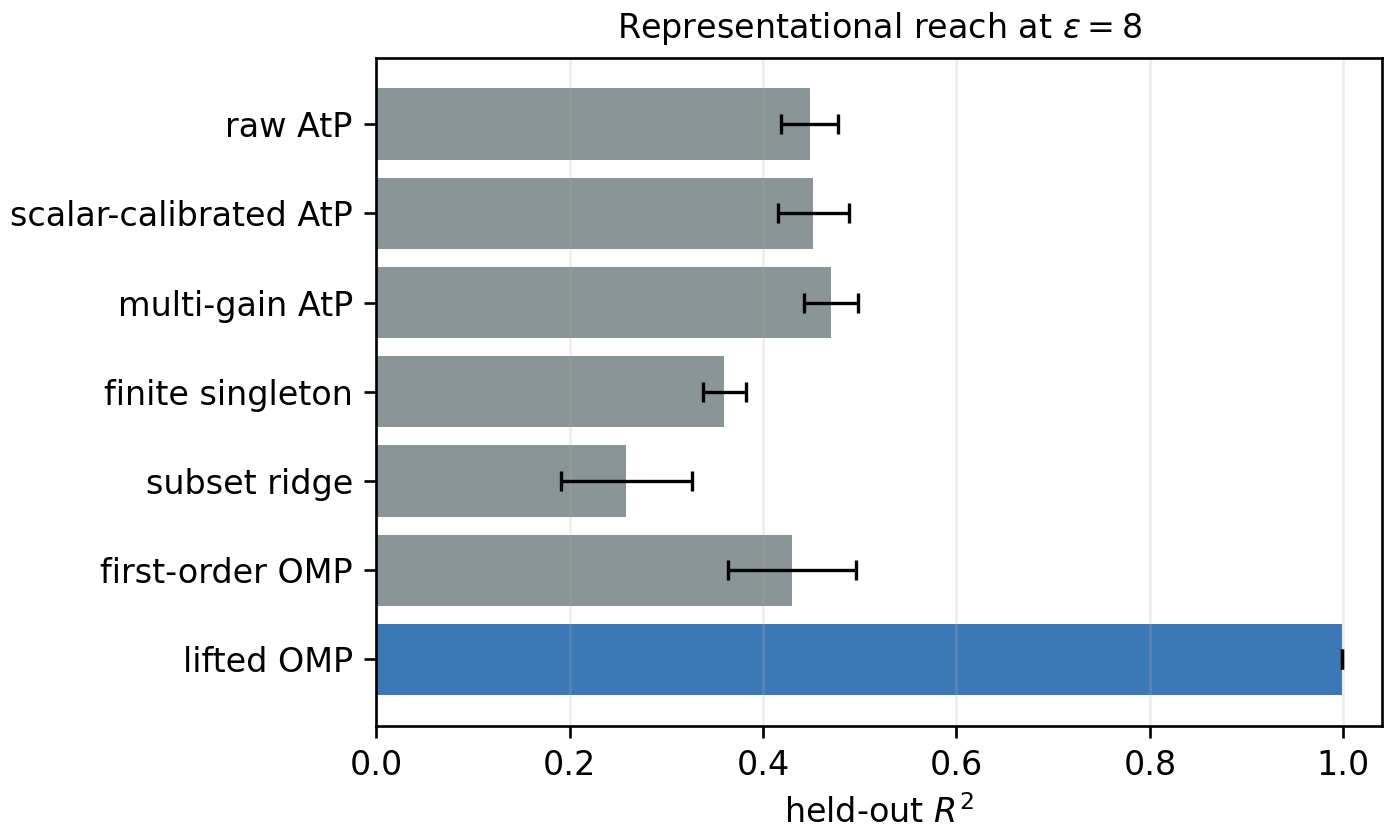
\includegraphics[width=0.92\linewidth]{figs/claim3_bar_bad.png}
\caption{Interaction-aware recovery at $\eps=8$ with a generous fixed budget. Lifted OMP recovers the planted pair-bearing response, while methods without pair features remain below $0.5$ held-out $R^2$.}
\label{fig:claim3bar}
\end{figure}

\paragraph{How many forward measurements are needed?}

Once we know that the lifted family can represent the response, we reduce the measurement budget. We require both held-out $R^2\ge0.95$ for finite-response prediction and pair recall $\ge0.99$ for the planted support. Lifted OMP first meets both conditions with 64 aggregate measurements at $\eps=5$ and 72 at $\eps=8$. Exhaustively measuring every pair would require 2,016 probes.

The usual sparse-recovery heuristic gives $4\log(N/4)\approx25$ measurements for four nonzero terms in 2,080 dimensions. We report this only for orientation. It omits constants, mask normalization, finite-sample variation, and the conditioning of the lifted design. Low-budget trials are also variable. We therefore report the first budget at which both prediction and support-recovery thresholds hold, rather than selecting the best isolated run.

\begin{figure*}[t]
\centering
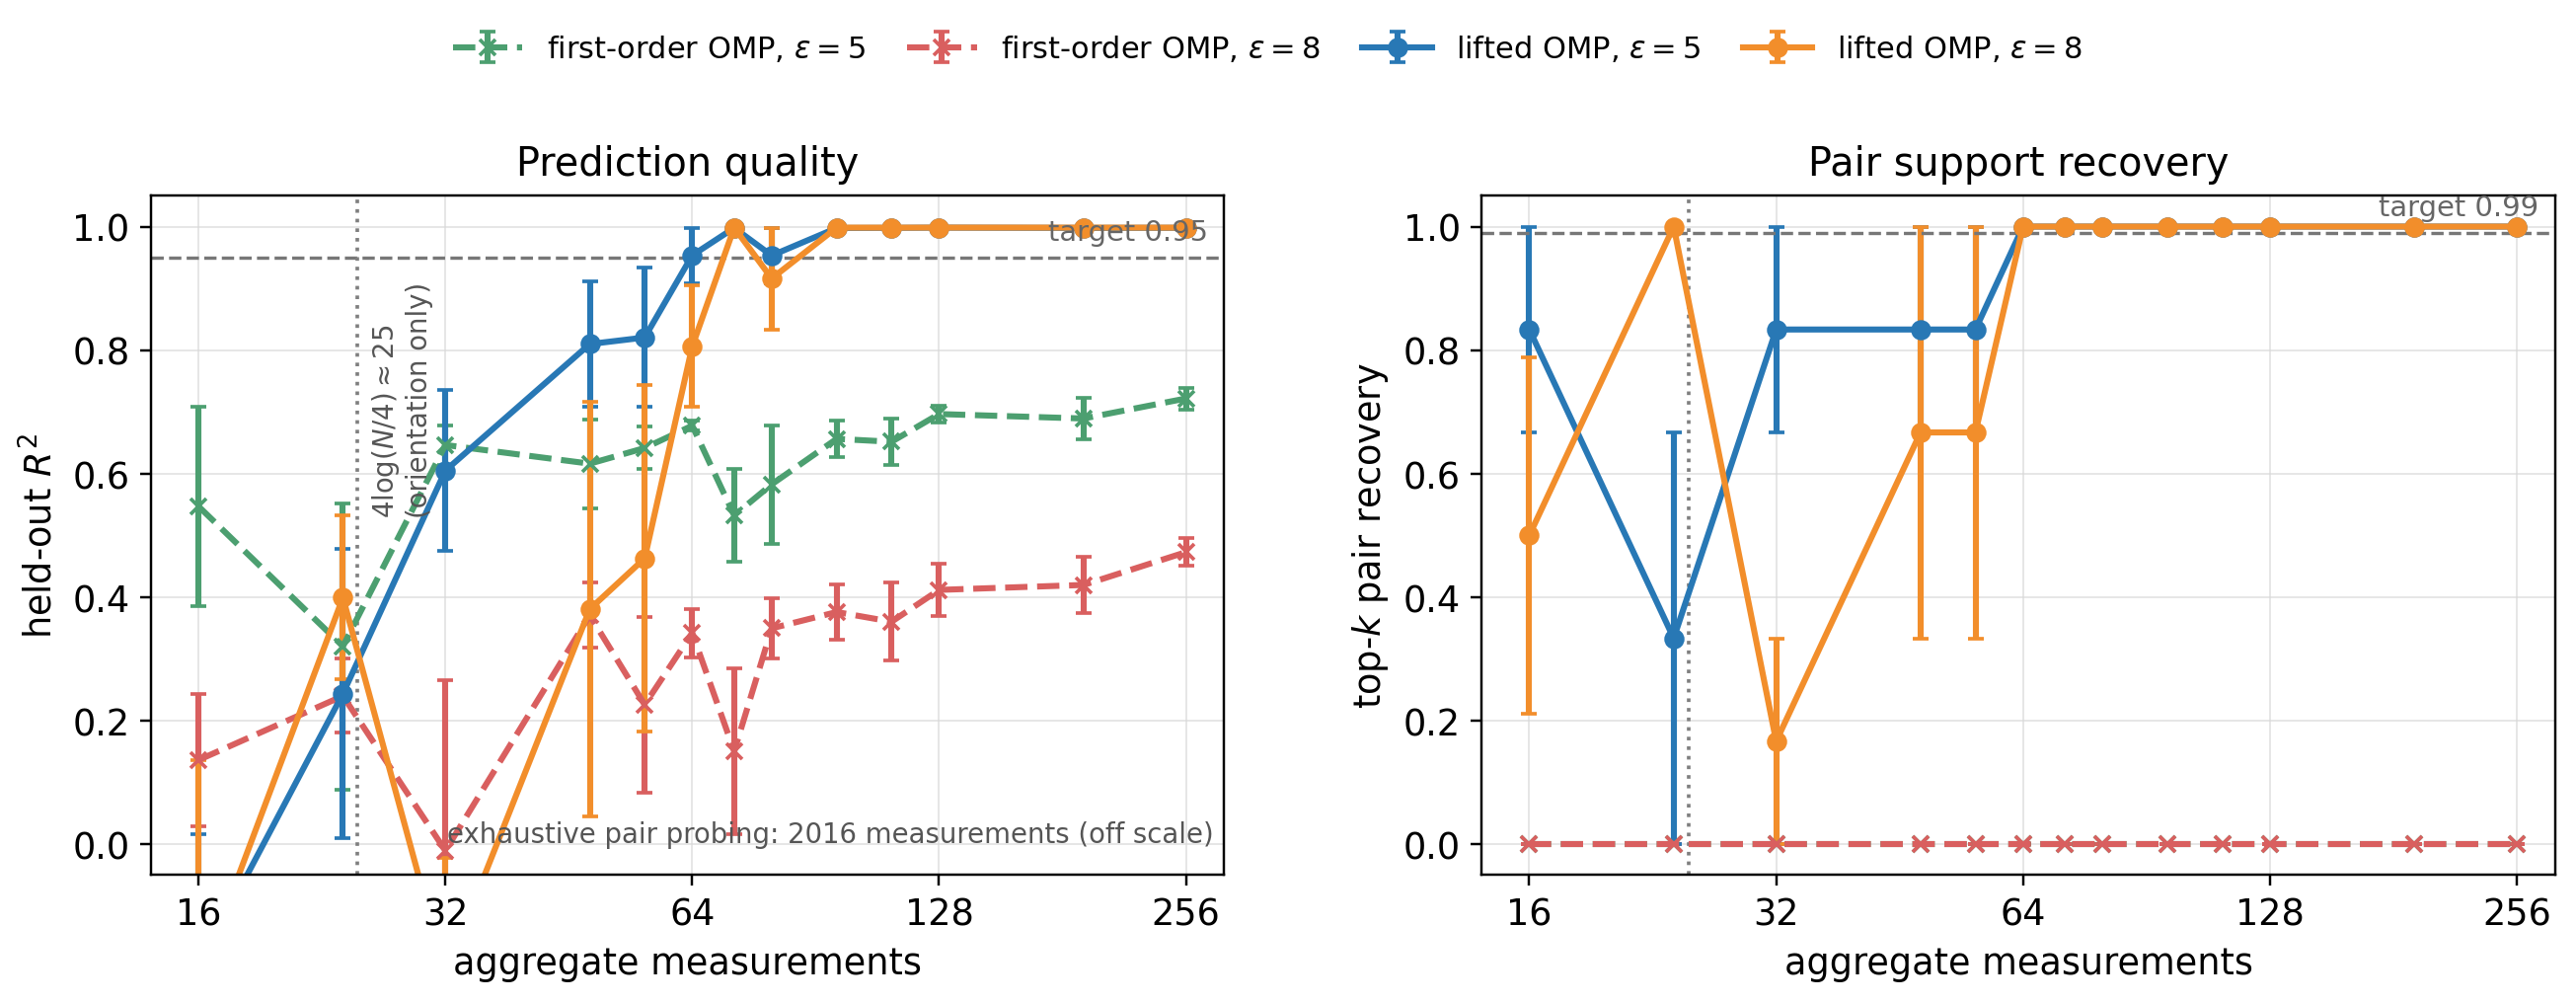
\includegraphics[width=0.92\textwidth]{figs/claim3_budget_clean.png}
\caption{Measurement budget for lifted recovery. With four planted nonzero terms among 2,080 main-and-pair features, lifted OMP reaches the prediction and pair-recall thresholds with 64--72 aggregate measurements, compared with 2,016 exhaustive pair probes. First-order OMP has no pair features.}
\label{fig:budget}
\end{figure*}

\paragraph{White-box alternative: AtP plus HVPs.}

Lifted forward measurements are useful when the endpoint is available only through model evaluations, as with sampling, decoding, retrieval, tool use, or a behavioral score. With white-box access, we can measure the local pair structure more directly. A gradient asks how the output initially changes along each component direction. An HVP asks how those gradient effects change when we move in a chosen direction. Attribution patching supplies the main-effect map in one backward pass, while designed HVP queries provide aggregate measurements of pair curvature.

The planted response is exactly quadratic. For this system, multiplying the local HVP pair coefficient by $\eps$ gives the normalized finite-scale pair coefficient. We know this conversion because we constructed the response function. We do not assume that the same conversion holds along a finite intervention path in a transformer.

The combined AtP--HVP observer reaches held-out $R^2\ge0.95$ and pair recall $\ge0.99$ with 12 HVP queries at $\eps=5$ and 24 at $\eps=8$. These are empirical thresholds for this harness, not a scaling law. They count the HVP queries; the full method also requires the AtP backward pass that supplies the main effects.

The pair-only HVP ablation finds the correct interacting pairs but reaches only $R^2=0.36$ at $\eps=5$ and $0.60$ at $\eps=8$. Recovering the pair support is therefore not enough to predict the full response. The observer must combine the AtP main effects with the HVP pair effects. Replacing the gradient main effects with finite singleton effects also performs worse. In this harness, singleton interventions saturate and underpredict larger aggregate changes, while the gradient remains the better main-effect approximation once the missing pairs are included.

\begin{figure*}[t]
\centering
\begin{subfigure}{0.49\textwidth}
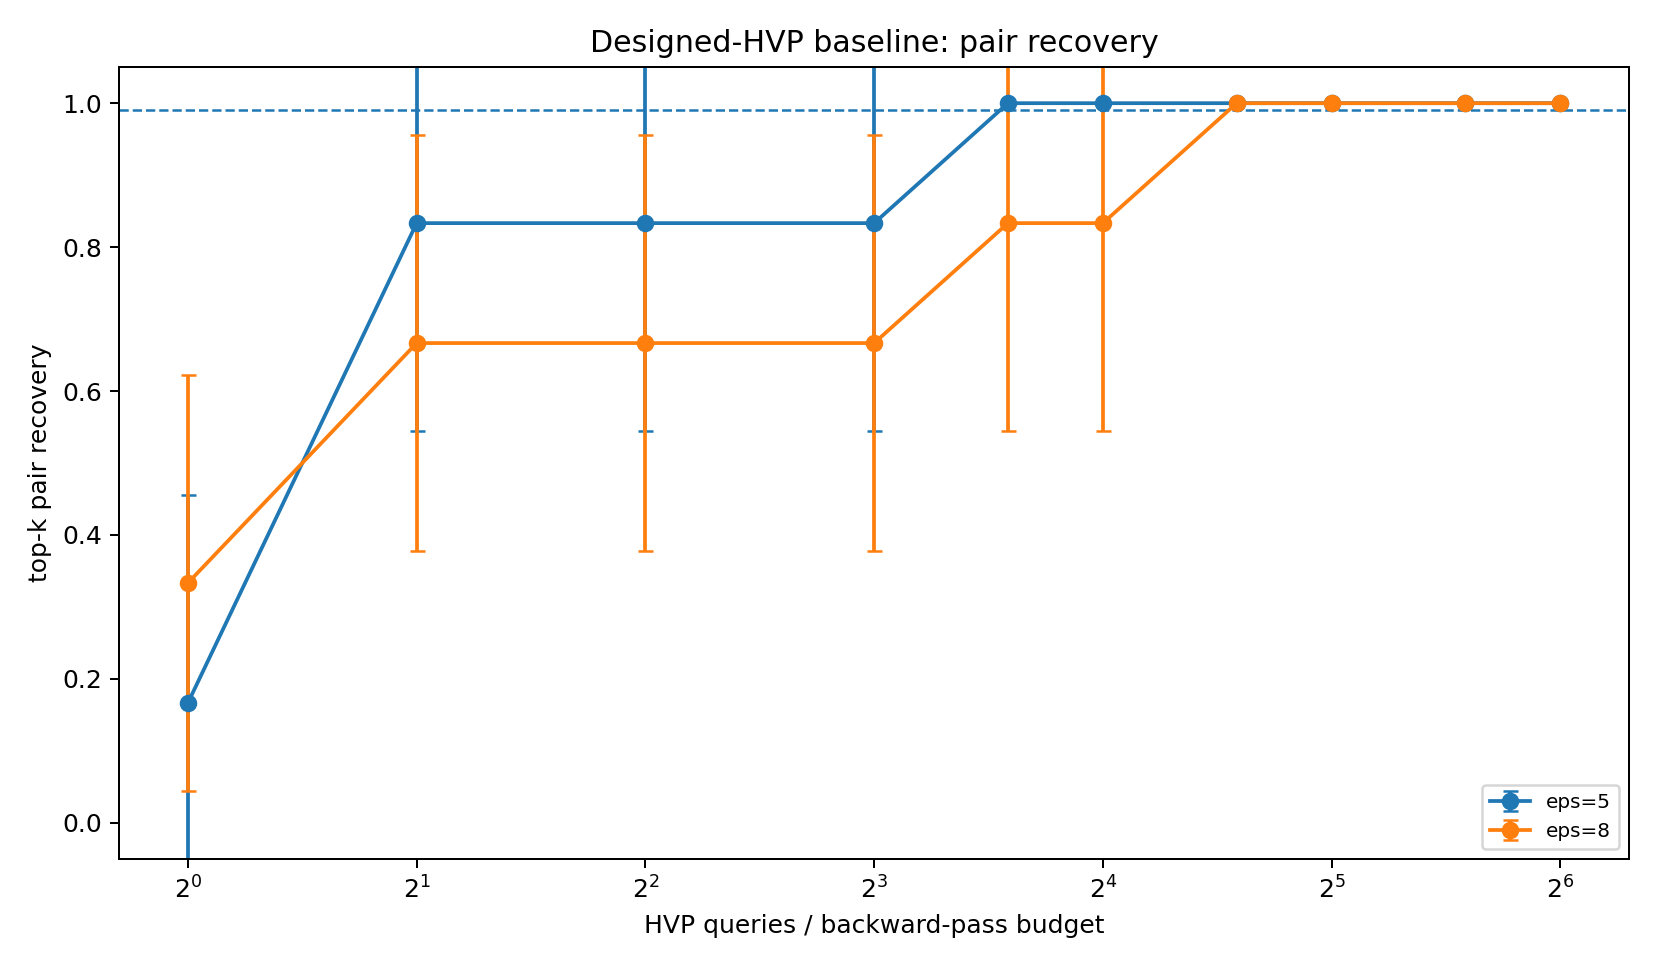
\includegraphics[width=\linewidth]{figs/claim3_hvp_pair_recall.png}
\caption{pair recovery}
\end{subfigure}\hfill
\begin{subfigure}{0.49\textwidth}
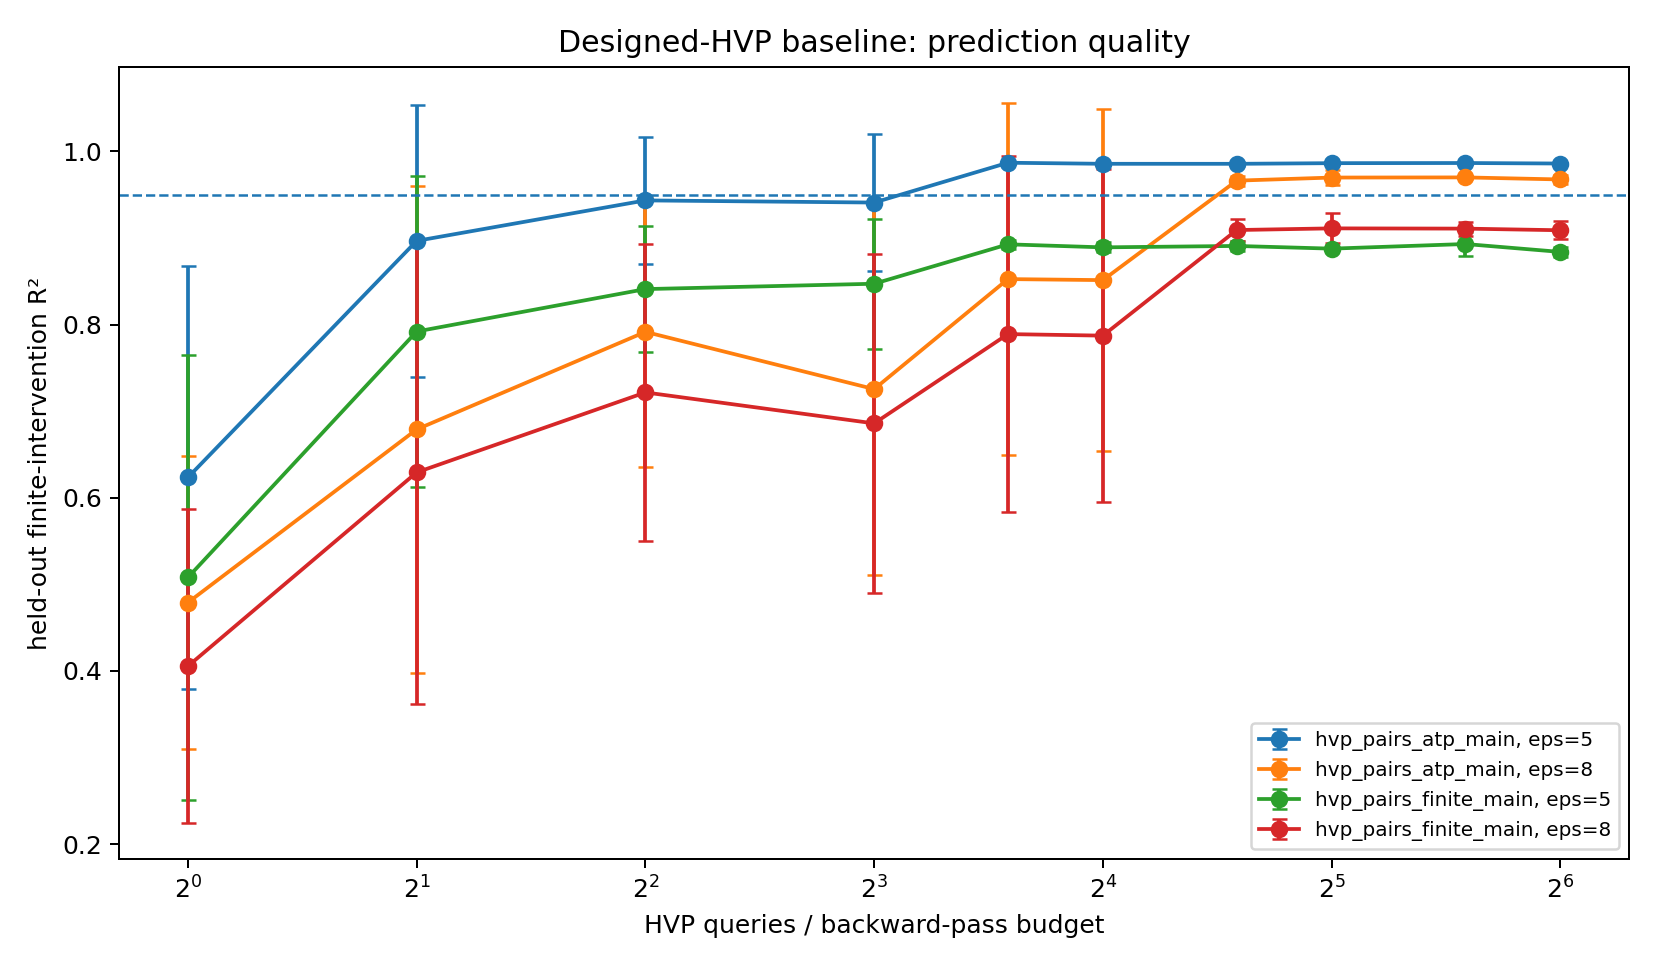
\includegraphics[width=\linewidth]{figs/claim3_hvp_r2.png}
\caption{held-out prediction}
\end{subfigure}
\caption{White-box interaction recovery. Designed HVPs recover the local pair map, and the quadratic harness supplies the known conversion to finite-scale pair coefficients. Accurate prediction also requires the AtP main-effect map.}
\label{fig:hvp}
\end{figure*}

\paragraph{Support recovery and response prediction are different.}

We next use 96 forward measurements, above the clean recovery threshold, and add zero-mean Gaussian noise to each normalized response. This separates two possible goals: locating the interacting pairs and estimating their coefficients accurately enough to predict a new intervention.

At $\eps=5$, both prediction and pair recall remain high through noise standard deviation $0.01$, while pair recall alone persists through $0.05$. At $\eps=8$, both remain high through $0.05$, and recall alone persists through $0.2$. The interacting pair can therefore remain identifiable after coefficient error has made the observer unsuitable for finite-response prediction.

\begin{figure*}[t]
\centering
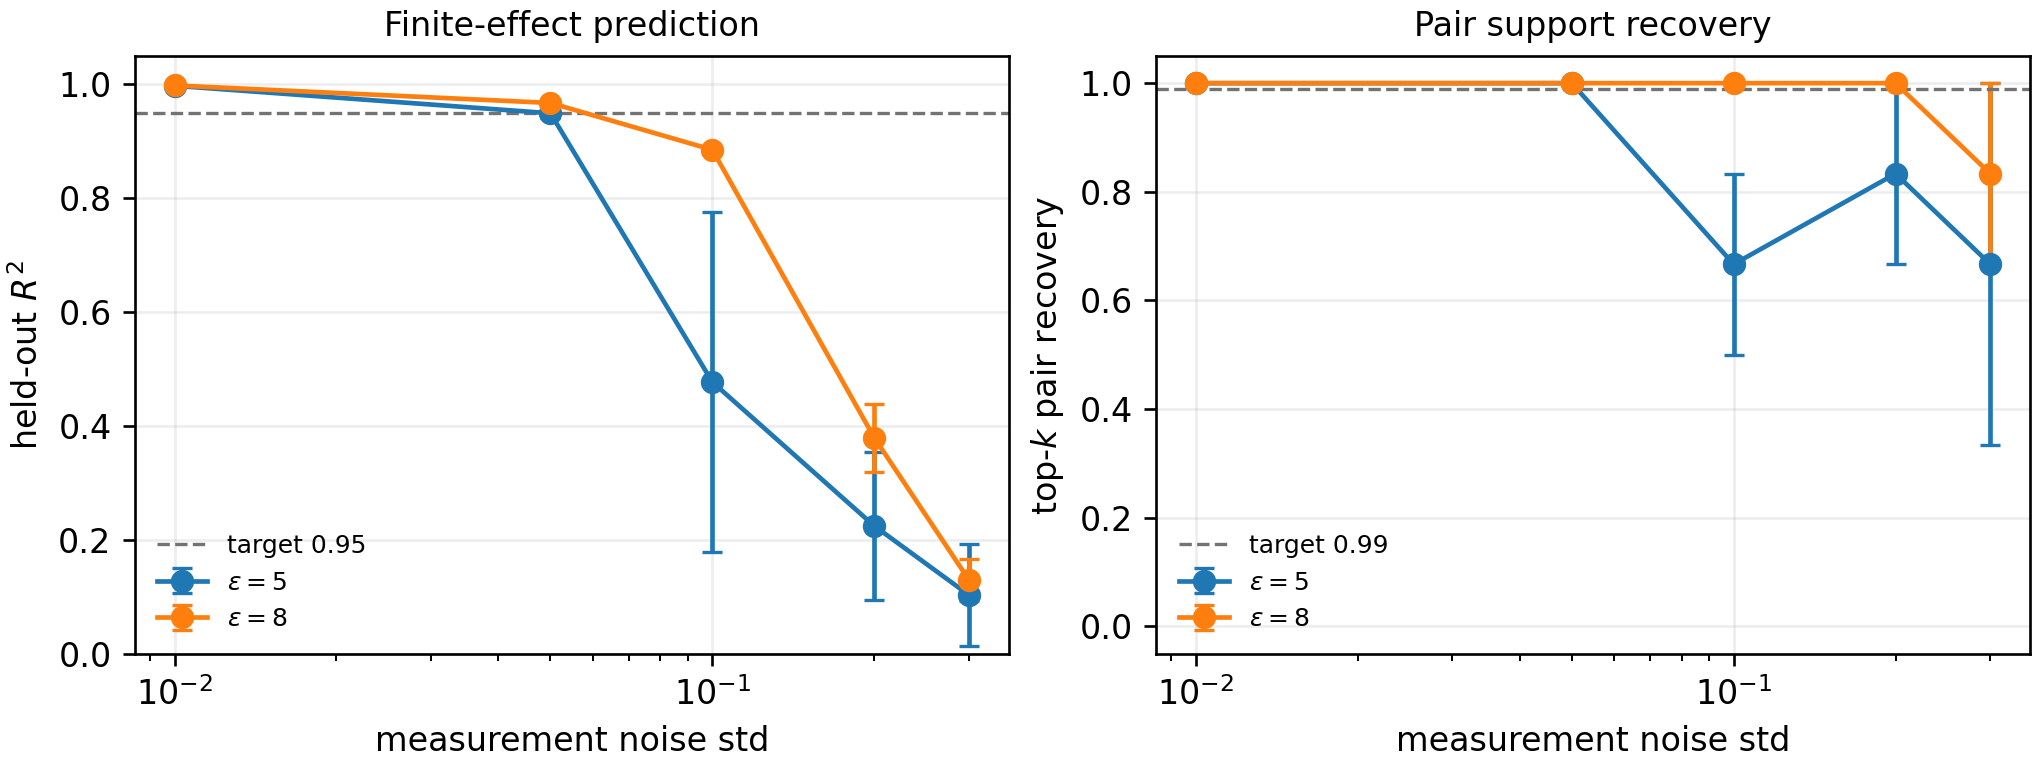
\includegraphics[width=0.92\textwidth]{figs/claim3_noise_clean.png}
\caption{Noise robustness with 96 aggregate measurements. Pair support can remain recoverable after held-out finite-response prediction degrades, separating support identification from coefficient accuracy.}
\label{fig:noise}
\end{figure*}

\paragraph{Why held-out masks matter.}

Finally, we give one off-path coordinate the same pattern as a causal coordinate on the training masks. Either feature can then explain the observed responses, even though only one belongs to the planted mechanism. This is a measurement alias.

Sparse support selection followed by independent held-out masks suppresses the false positive. The test shows why held-out interventions participate in identification rather than serving only as a final score. It does not exhaust the problem: a stronger future stress test should alias a false pair with a true pair inside the lifted design.

The planted harness shows when interaction-aware measurements are necessary and how forward-only and white-box access lead to different recovery routes.



\subsection{The basis determines the required measurement family}\label{sec:basis}

The planted experiment in Sec.~\ref{sec:interactions} gives us the correct coordinates in advance. Real interpretability work does not. The same computation can look additive in a basis that contains a completed detector and interactional in a basis that contains only the detector's inputs. We therefore need a system in which we can change the basis while keeping the underlying computation known.

A simple conjunction illustrates the issue. Suppose the model must report whether the previous token is A and the current token is B. If the basis contains one completed ``AB detected'' coordinate, an additive readout can use that coordinate directly. If the basis contains only separate coordinates for ``previous token is A'' and ``current token is B,'' neither coordinate is sufficient by itself. Their product is required. The computation has not changed; only the coordinates used to describe it have changed.

Tracr provides this intermediate setting~\cite{lindner2023tracr}. It compiles programs written in the restricted-access sequence processing (RASP) language into executable transformers. The compiler also assigns names to residual-stream coordinates associated with program variables. We can therefore inspect the same known computation through different sets of coordinates.

We compile three programs over the symbols A, B, and C. The first reports a property of the current token and serves as an additive control. The other two detect the sequence pattern ``A followed by B.'' One uses a numeric representation and the other a boolean representation. Both compute the same conjunction but place it in different compiler-generated coordinates.

At sequence length 6, we enumerate all 243 possible input sequences. After excluding the position with no predecessor, this gives 1,215 position-level examples. We compare two bases. The \emph{native} basis contains the full set of compiler variables, including the completed AB detector. The \emph{restricted} basis contains only variables available before the conjunction has been formed, such as the current-token and previous-token labels.

\paragraph{Does the apparent interaction order change with the basis?}

For the current-token control, an additive model is sufficient in either basis. Both the full native basis and the token-only basis reach held-out position-level $R^2=1.0$.

The AB detectors are also additive in the native basis. This does not mean that the conjunction has disappeared. The compiler has already created an explicit coordinate that records whether ``A followed by B'' is true. Once that completed detector is available as one coordinate, an additive readout can use it directly.

The result changes in the restricted basis. This basis contains the current-token and previous-token information but no completed AB detector. An additive model explains only about half of the detector variance. Adding pair products restores held-out $R^2=1.0$ and selects the intended term:
\[
\text{previous-token-A}\times\text{current-token-B}.
\]
The underlying program has not changed. Only the coordinates have changed. The AB computation is first-order in the native basis and interactional in the restricted pre-conjunction basis.

\begin{figure}[t]
\centering
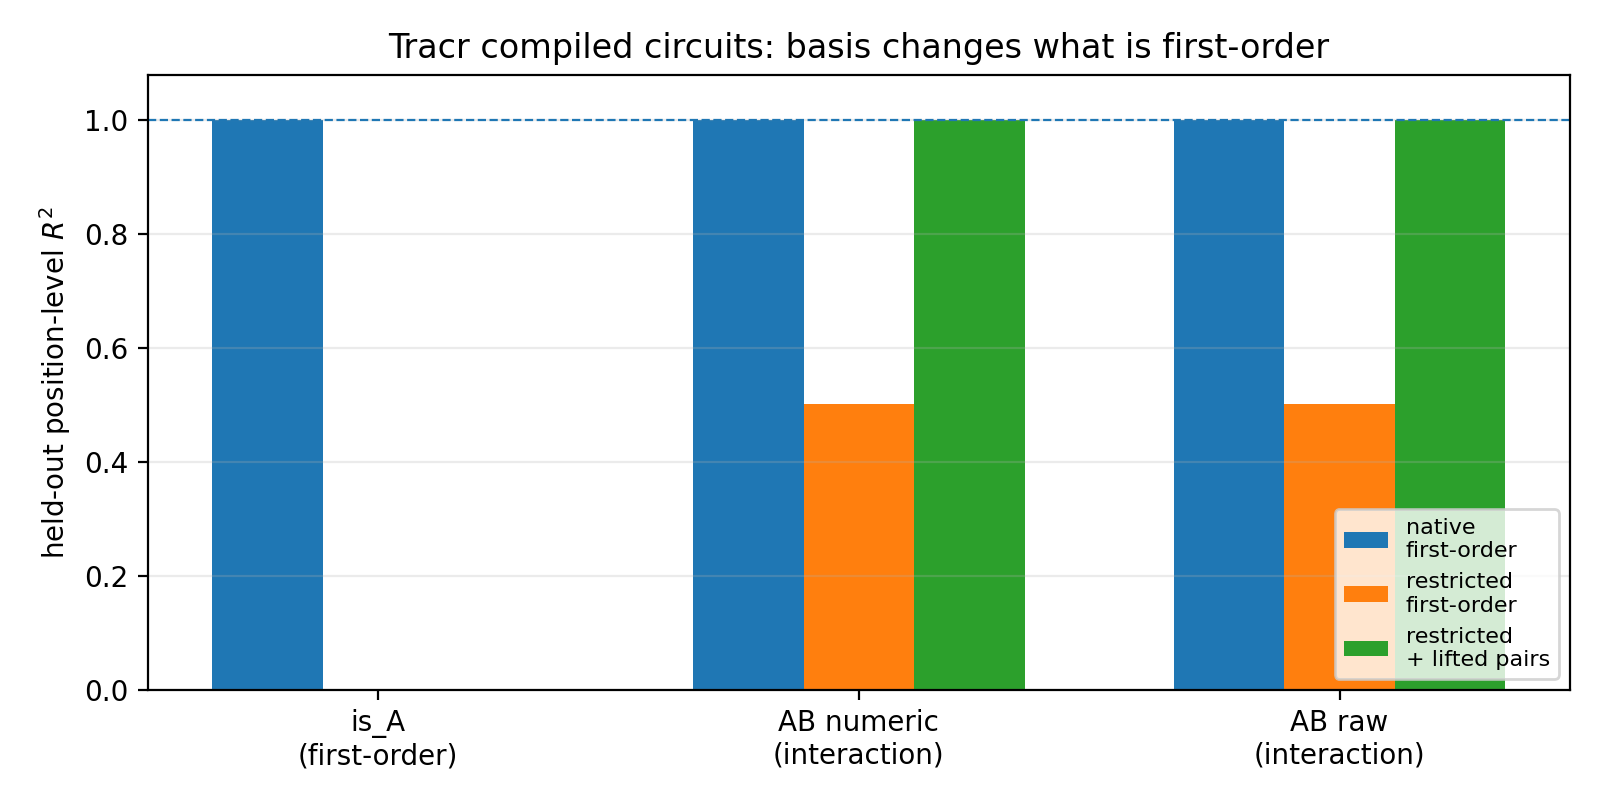
\includegraphics[width=0.95\linewidth]{figs/tracr_label_basis_clean.png}
\caption{Basis comparison in Tracr circuits. The current-token control is additive in both bases. The AB detectors are additive in the native compiler basis because it contains an explicit detector coordinate. In the restricted pre-conjunction basis, additive features explain only about half the variance, while lifted pair features recover the intended conjunction and restore held-out $R^2=1.0$.}
\label{fig:tracr}
\end{figure}

\paragraph{Does the readout use the reconstructed detector?}

Predicting a compiler label does not show that the model's output depends on it. We therefore intervene in the final residual stream, immediately before the readout. The numeric detector group contains the detector and its AB/OTHER coordinates. The boolean group contains the True/False detector and map coordinates.

We first ablate the detector group. We then reconstruct it from the restricted pre-conjunction basis using either additive features or lifted pair features and write that reconstruction back into the residual stream. This tests whether the recovered detector supplies information that the final readout actually uses.

The intervention location is deliberate. By editing the final residual stream, we isolate the connection between the detector subspace and the readout. We do not claim that the same reconstruction would survive the remaining transformer computation if it were written into an earlier layer.

Ablating the detector group drops held-out readout $R^2$ from $1.00$ to about $-0.05$ for the numeric program and $-0.51$ for the boolean program. The final output therefore depends on these detector coordinates. Writing back the additive reconstruction restores readout $R^2$ to only about $0.55$ for both programs. Writing back the lifted reconstruction restores the original $R^2=1.00$.

The same pattern appears when we score reconstruction of the detector group itself. Additive features reach about $.68$ for the numeric group and $0.93$ for the boolean group. Lifted features reconstruct both groups perfectly. The apparently high additive score for the boolean group is misleading: it mostly captures the common negative case and misses the rare positive conjunction that matters to the output.

The negative $R^2$ after boolean ablation also has a simple explanation. The boolean group contains complementary True and False coordinates. Setting both to zero creates a state that never occurs during normal execution. The readout must extrapolate from this out-of-distribution state and performs worse than a constant mean predictor. This is an ablation artifact, not evidence that the detector is harmful.

\begin{figure*}[t]
\centering
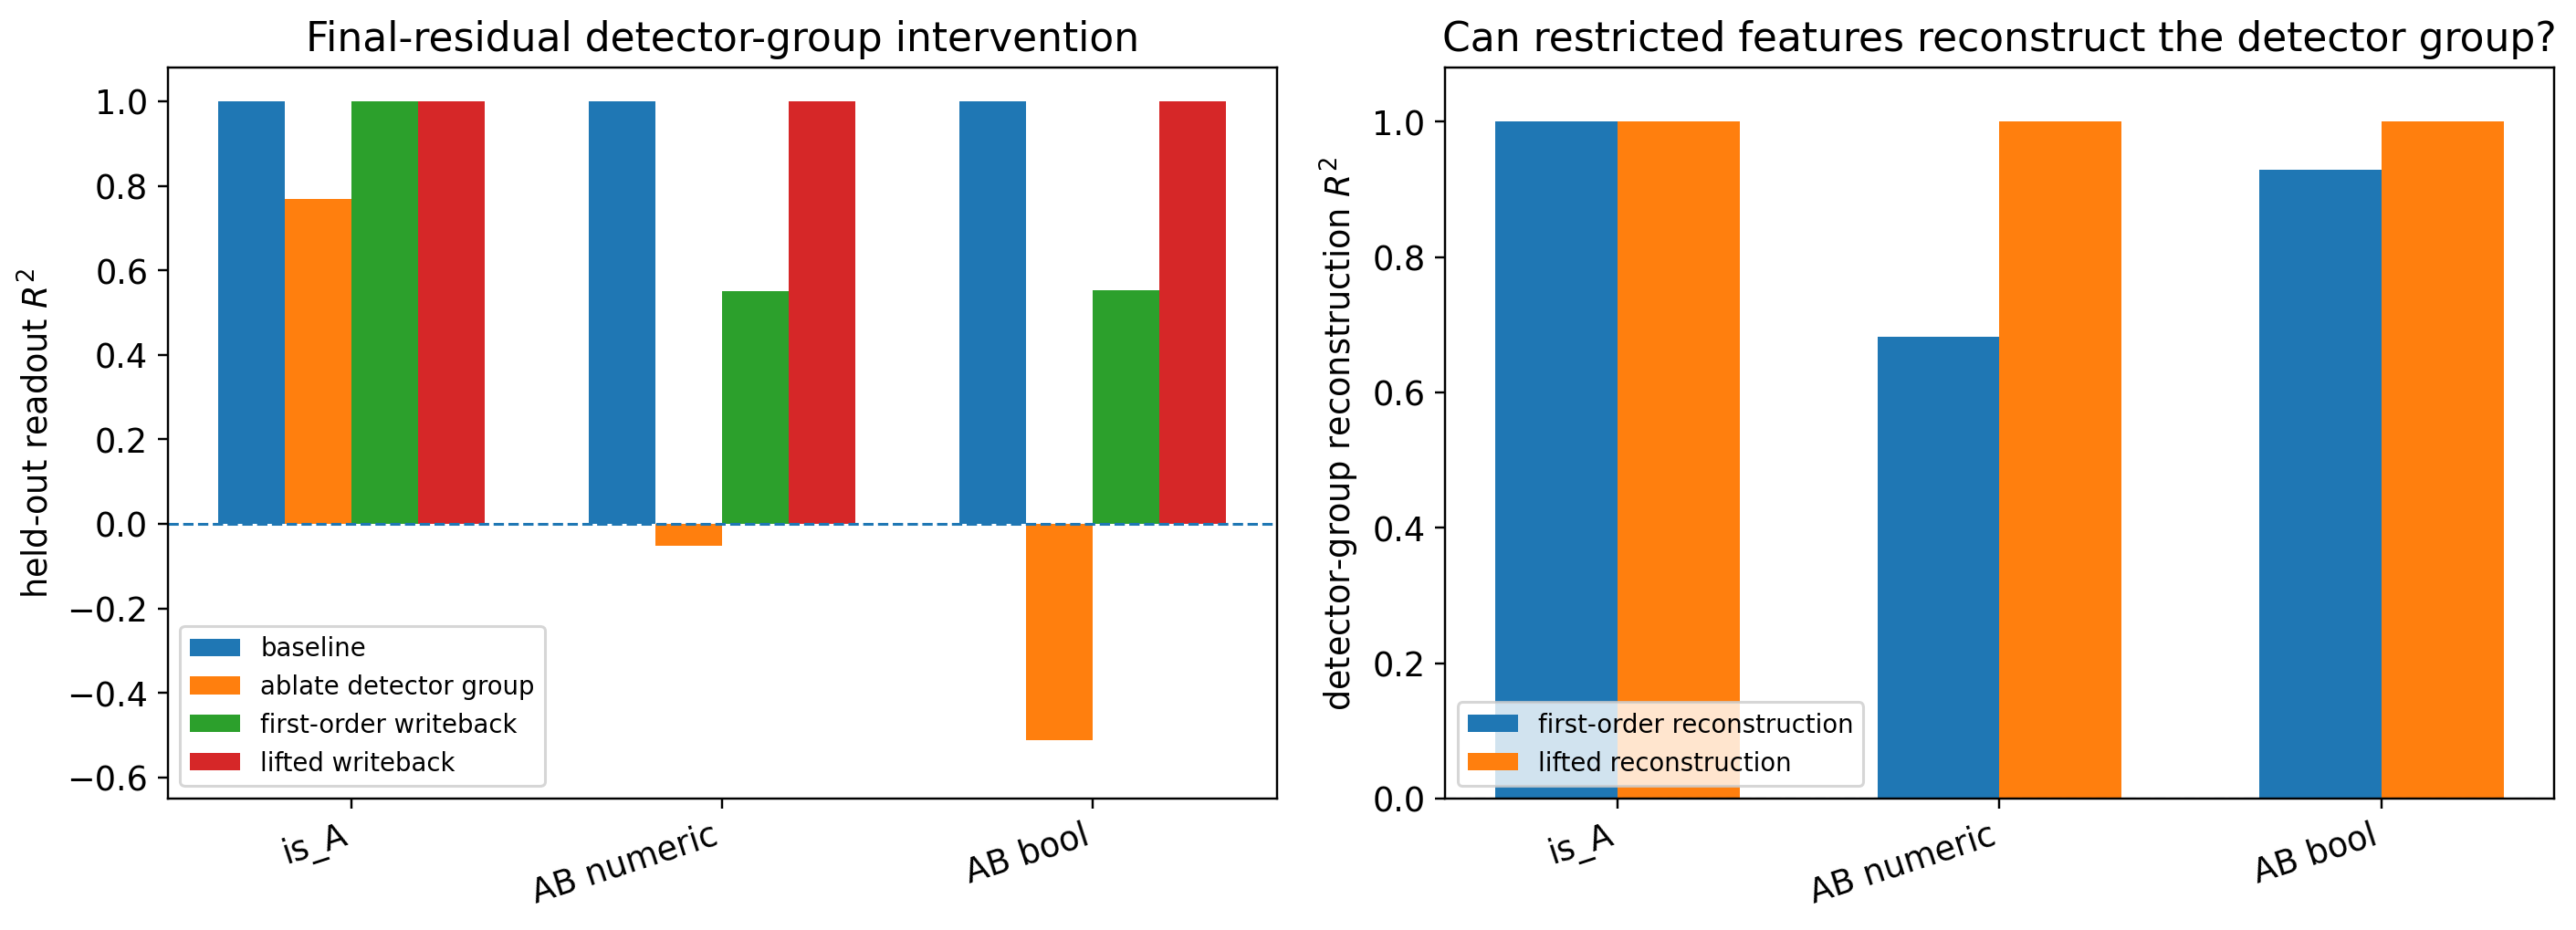
\includegraphics[width=0.98\textwidth]{figs/tracr_group_intervention_clean.png}
\caption{Detector-group writeback in Tracr circuits. Left: ablating the final-residual detector group destroys output prediction for the AB programs, while writing back the lifted reconstruction restores the original held-out $R^2$. Right: additive features only partially reconstruct the detector groups, whereas lifted features reconstruct them completely.}
\label{fig:tracr_group}
\end{figure*}

The conclusion is direct. The AB computation is additive in a basis that contains its completed detector, interactional in a basis that contains only its inputs, and additive again after those inputs are lifted with pair features. The writeback test shows that the recovered detector subspace is used by the final readout.

\subsection{IOI reproduces conditional backup and ranks the primary--negative interaction first}\label{sec:ioi}

Tracr lets us check an observer against compiler labels and a known program. A pretrained language model removes that ground truth. We therefore end with the indirect-object identification (IOI) task in GPT-2-small. Prior work has identified a circuit for this task and documented several qualitative behaviors, including a conditional backup response~\cite{wang2022ioi,mcdougall2023copy}. This gives us a useful intermediate case: we know which groups to examine and roughly what they do, but we do not know the finite effect of every possible intervention.

Consider the prompt ``When Alice and Bob went to the store, Alice gave a book to \ldots''. The model should predict Bob, the indirect object (IO), rather than Alice, the repeated subject (S). Three documented head groups contribute to this choice. Primary Name Movers write evidence for Bob toward the output. Backup Name Movers provide another route for writing Bob and become important when the primary route is weakened. Negative Name Movers are different: they write a negative signal against names that earlier components have already begun to copy. They act as a copy-suppression or calibration mechanism rather than as another answer-writing path~\cite{mcdougall2023copy}. On the IOI intervention surface studied here, their net effect lowers the IO-versus-subject readout, so removing them can improve that particular readout.

Let $P$ denote the three primary Name Mover heads $(9.9,\allowbreak 9.6,\allowbreak 10.0)$, $B$ the eight Backup Name Movers $(9.0,\allowbreak 9.7,\allowbreak 10.1,\allowbreak 10.2,\allowbreak 10.6,\allowbreak 10.10,\allowbreak 11.2,\allowbreak 11.9)$, and $E$ the two Negative Name Movers $(10.7,\allowbreak 11.10)$. A label such as $9.9$ means layer 9, head 9. We measure the final-token margin
\[
M=\logit(\mathrm{IO})-\logit(\mathrm{S}).
\]
In the example, $M>0$ means that Bob ranks above Alice, while $M<0$ means that Alice ranks above Bob. A change in $M$ does not necessarily change the emitted token: the output flips between these two names only if the margin crosses zero, and another vocabulary token could also rank above both.

For an ablated set of heads $U$, let $\Delta(U)$ be the clean margin minus the ablated margin. Positive $\Delta(U)$ means that the ablation moves the model away from Bob and toward Alice. Negative $\Delta(U)$ means that it moves the model toward Bob.

We use two studies because complete group ablations and prediction over ordinary subset masks answer different questions. The direct study uses 21 selected group masks, 128 matched name pairs, and eight prompt conditions formed by four lexical frames in the standard ABBA and BABA orders. These two orders reverse how the names are introduced relative to the person who later repeats as the subject. We repeat the study with two ablation conventions. Template-conditioned mean ablation replaces a selected head output with its average clean activation on that prompt template; zero ablation replaces it with zero. Agreement across the two reduces the chance that the interaction ordering comes from one replacement convention. This study asks what happens at the corners of the intervention space, where whole groups are removed.

The predictive study measures 240 masks over 256 name pairs on one prompt template. A masked head is replaced by its average clean activation on prompts from that template. We score the 239 non-clean masks using five folds, while retaining the clean mask as an anchor in every training fold. This study asks which measurement model best predicts unseen subset interventions drawn from the tested mask distribution.

\paragraph{Direct group ablations reproduce conditional backup.}

For two groups $A$ and $B$, define
\[
I_{AB}=\Delta(A+B)-\Delta(A)-\Delta(B).
\]
If their effects add independently, $I_{AB}=0$. A positive value means that removing both groups causes more damage than we would predict by adding their separate effects.

The primary and backup groups give a concrete example. On the original template, removing $P$ lowers the Bob--Alice margin by $0.463$, while removing $B$ lowers it by $0.350$. An additive model therefore predicts that removing both groups will lower the margin by $0.813$. The measured reduction is instead $1.869$, giving $I_{PB}=1.055$.

In terms of the prompt, the backup path looks relatively unimportant while the primary heads are still writing Bob. Once the primary path is gone, losing the backups becomes much more damaging. For illustration, suppose the clean model favors Bob by $1.5$ logits. The additive estimate predicts that Bob will remain ahead by $0.687$ after both groups are removed. The measured joint effect instead gives a margin of $-0.369$, placing Alice ahead of Bob. The value $1.5$ is illustrative, but it shows what the interaction means for an actual prediction: an additive observer can put the model on the wrong side of the Bob--Alice decision boundary.

The Negative Name Movers produce a different sign. Averaged over the eight lexical/order conditions, mean ablation gives $\Delta(E)=-2.270$ and $\Delta(P+E)=-0.136$; zero ablation gives $-2.335$ and $-0.769$. Removing $E$ alone therefore improves the IO-versus-subject margin. This is consistent with copy suppression: a mechanism that improves calibration over the broader model distribution can still oppose a narrow task-specific logit difference.

\begin{table}[t]
\centering
\caption{Direct IOI group interactions across four lexical frames in ABBA and BABA order, with 128 shared matched name pairs. Intervals use a crossed bootstrap that resamples lexical frames and one shared name-pair vector while retaining both orders. The last column divides by the number of possible cross-group head pairs; it does not assign the same effect to every individual pair.}
\label{tab:ioi-direct}
\scriptsize
\setlength{\tabcolsep}{2pt}
\begin{tabular}{@{}lccc@{}}
\toprule
Pair (heads) & \shortstack{mean ablation\\$I$ [95\%]} & \shortstack{zero ablation\\$I$ [95\%]} & \shortstack{$I$/pair\\(mean/zero)} \\
\midrule
$P\times B$ (24) & 1.080 [.912, 1.262] & 1.268 [1.013, 1.558] & 0.045/0.053 \\
$P\times E$ (6)  & 1.830 [1.569, 2.076] & 1.681 [1.474, 1.889] & 0.305/0.28 \\
$B\times E$ (16) & .502 [0.429, 0.576]    & 0.518 [0.416, 0.618]    & 0.031/0.032 \\
\bottomrule
\end{tabular}
\end{table}

\paragraph{The primary--negative interaction is larger.}

The $P\times E$ result also has a direct interpretation in the Alice--Bob example. Under mean ablation, removing the primary heads lowers the Bob--Alice margin by about $0.304$. Removing the Negative Name Movers while leaving the primary path intact raises the margin by $2.270$. If these effects were independent, removing both groups would raise the margin by
\[
2.270-0.304=1.966.
\]
The observed increase is only $0.136$.

The reason is conditional copy suppression. While the primary heads are writing Bob, the Negative Name Movers have a strong copied-name signal to act against. Removing the negative heads then releases that suppression and gives Bob a large boost. Once the primary heads have also been removed, much less Bob evidence remains for the negative heads to suppress. Removing them therefore provides almost no boost. The difference between the predicted and observed responses, $1.830$ logits, is the measured $P\times E$ interaction.

Every tested lexical/order condition gives the same ordering, $PE>PB>BE$, under both ablation conventions. The $PE-PB$ contrast is $0.750$ [$0.562,0.934$] under mean ablation and $0.413$ [$0.207,0.611$] under zero ablation. Both contrasts remain positive when we remove any one lexical frame.

The difference is not an artifact of group size. After dividing by the number of possible cross-group head pairs, the normalized $PE$ effect is $6.8\times$ the normalized $PB$ effect under mean ablation and $5.3\times$ under zero ablation.

These pair terms are not a complete circuit decomposition. A three-way residual of $0.319$ [$0.215,0.439$] remains under mean ablation, and $0.601$ [$0.417,0.790$] remains under zero ablation. Table~\ref{tab:ioi-direct} therefore ranks three documented group interactions. It does not assign all circuit behavior to pairs or claim that every individual $P$--$E$ head pair has the same effect.

\paragraph{Held-out subset prediction gives the same ordering.}

The predictive study asks whether these interactions help predict unseen subset masks, rather than only complete group ablations. We stratify masks by the exact number of removed primary heads, a binned count of removed Backup Name Movers, and the exact number of removed Negative Name Movers. We oversample masks with at least two removed primary heads because conditional backup is most visible after the primary path has been weakened.

A count-additive baseline gives each group its own flexible dose response. It can learn, for example, that removing four backup heads has more than twice the effect of removing two. What it cannot express is that removing a Negative Name Mover helps Bob while the primary writers remain but helps much less after those writers have been removed.

We represent that dependence by adding one normalized count product at a time:
\[
q_Pq_B,\qquad q_Pq_E,\qquad q_Bq_E,
\]
where $q_P=n_P/3$, $q_B=n_B/8$, and $q_E=n_E/2$. These are interactions between group-level ablation counts, not between identified pairs of individual heads.

The count-additive baseline has MAE $.386$ and $R^2=0.752$. A per-head additive check gives similar values: MAE $0.379$ and $R^2=0.759$. Adding the $PB$, $PE$, or $BE$ term gives MAE $0.377$, $0.259$, and $0.386$, respectively, and $R^2=0.774$, $0.887$, and $0.754$.

Across 2,000 paired prompt bootstraps with fixed five-fold splits, $PB$ improves MAE by $0.0083$ (95\% CI $[0.0064,0.0101]$), while $PE$ improves it by $0.1265$ (95\% CI $[0.1195,0.1338]$). The $BE$ change is $-0.0002$ (95\% CI $[-0.0015,0.0011]$), which is indistinguishable from no improvement. Adding all three terms gives MAE $0.236$, $R^2=0.907$, and an MAE improvement of $0.1499$ (95\% CI $[0.1425,0.1578]$).

The ordering also survives changes to the fold assignment. The $PE$ gain is positive in all 200 audited assignments, $PB$ in 199, and $BE$ in 154. Among the three tested single interaction terms, $PE$ is therefore both the largest and the most stable. $PB$ gives a smaller but repeatable gain, while $BE$ is split-sensitive.

\begin{figure}[t]
\centering
\begin{subfigure}{0.48\linewidth}
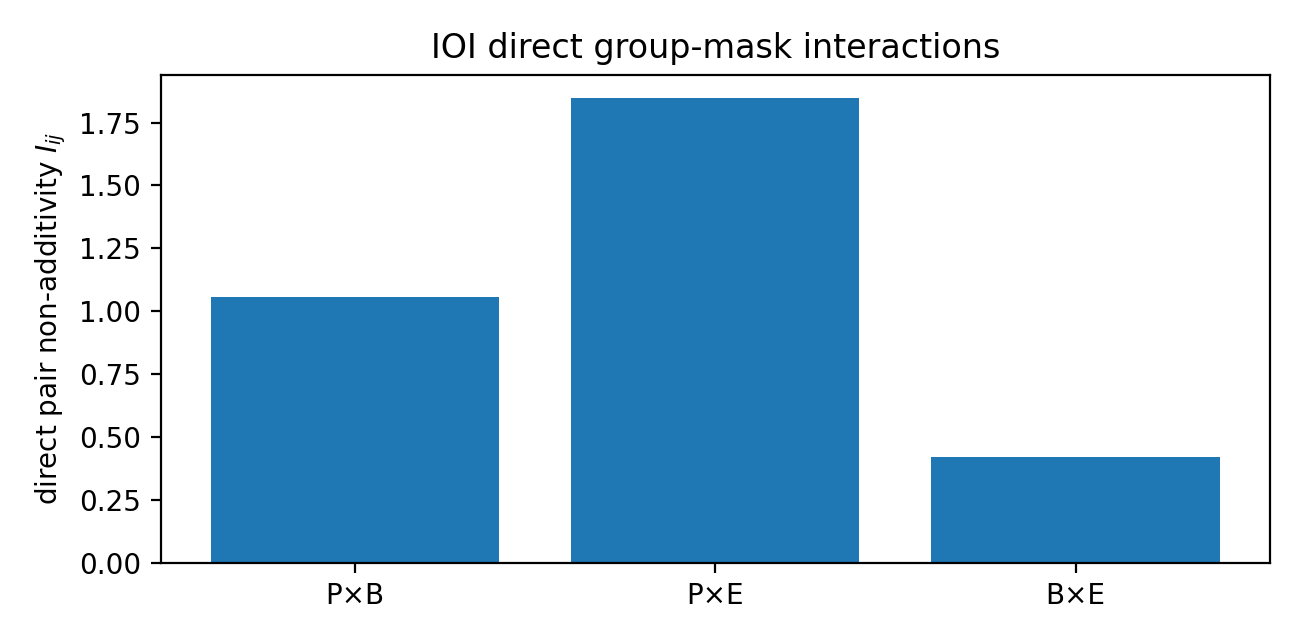
\includegraphics[width=\linewidth]{figs/ioi_direct_group_interactions.png}
\caption{Direct group-mask interactions}
\end{subfigure}\hfill
\begin{subfigure}{0.48\linewidth}
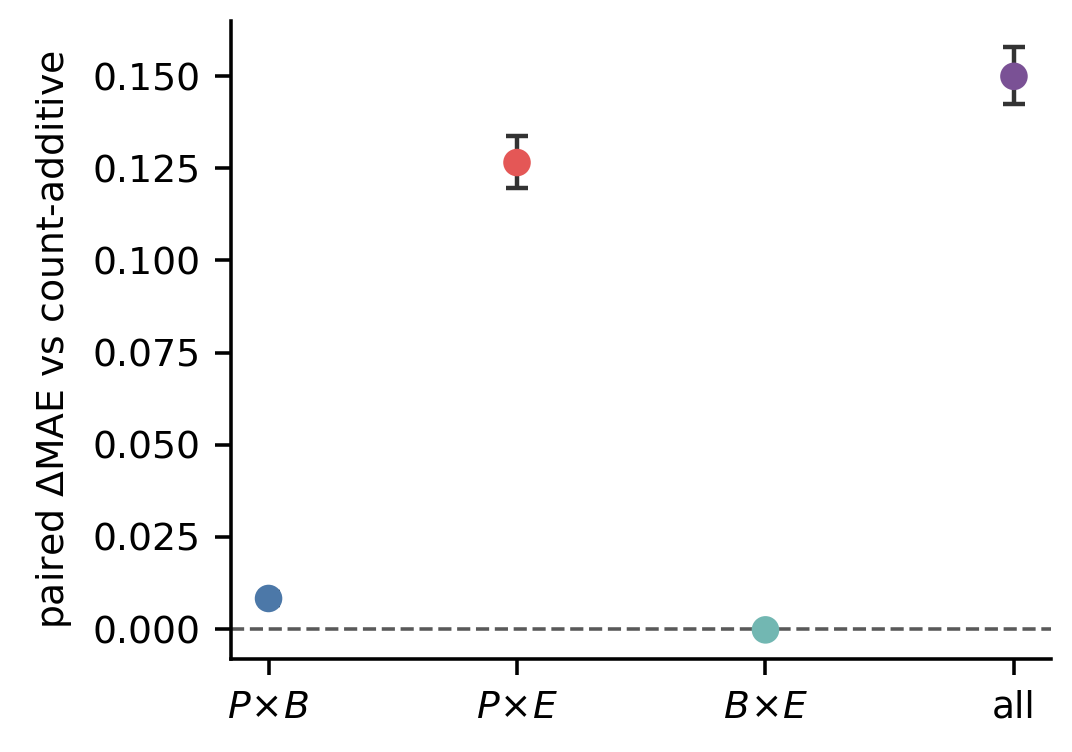
\includegraphics[width=\linewidth]{figs/ioi_predictive_consistent_seed.png}
\caption{Held-out prediction gain}
\end{subfigure}
\caption{IOI interaction measurements. Left: direct group interactions on the original-template mean-ablation surface. Right: held-out gains from adding one count-product term to the count-additive model. $P\times E$ gives the largest of the three tested gains; the interval for $B\times E$ crosses zero.}
\label{fig:ioi-anchor}
\end{figure}

\paragraph{What mechanistic tomography adds.}

Prior IOI work supplies the candidate head groups and their qualitative roles. Mechanistic tomography supplies the procedure for testing whether those groups are sufficient for the intended prediction task. We first fit the additive family and test it on held-out interventions. Its residual shows that separate group effects cannot predict the finite response, so we lift the design with the three group-pair terms. The $P\times E$ column expresses that removing Negative Name Movers has one effect while the primary path remains and another after it has been weakened; adding it reduces held-out MAE from $0.386$ to $0.259$. MT does not discover the IOI groups. It identifies when the additive family has reached its limit and which relations among the documented groups are needed to predict finite interventions under the declared distribution.

\paragraph{What the two measurements tell us.}

The direct and predictive studies agree on the ordering of the three tested interactions, but they should not be treated as interchangeable. A complete $P+B$ ablation measures the corner where both groups are gone. A predictive term measures how useful that interaction is across the subset masks the observer will encounter. A strong corner interaction can make only a small average predictive contribution if the measurement distribution rarely approaches that corner.

This distinction explains why the known $P\times B$ backup response can be clear under complete group ablation yet add much less predictive value than $P\times E$ over the tested subset distribution. It also states the limit of the claim. We find that $P\times E$ is the strongest and most stable of three group-level interaction terms under the tested design. We do not identify a particular head pair as the dominant circuit edge, and the predictive comparison remains limited to one prompt template and mean ablation.

This is where complete mechanism ground truth runs out. Even so, the same questions remain useful: what intervention distribution will the observer face, which interaction family predicts responses from that distribution, and which conclusions survive changes in prompts and ablation conventions? The IOI study shows why all three must be stated.

\subsection{Finite calibration is sufficient on the tested Qwen-2.5-7B surface}\label{sec:qwen}

The preceding experiments use exact posteriors, planted effects, compiler labels, or documented circuit groups. We next ask whether the operational procedure can still be used when none of those references is available. This is a weaker test: it cannot tell us whether an observer has recovered the model's mechanism. It can still tell us whether the observer predicts the finite responses it was built to support.

We fix Qwen-2.5-7B-Instruct~\cite{qwen2025report} and a refusal-margin readout. The readout compares the model's log probability of four refusal stems with its log probability of four compliance stems at the first generated position. Harmful prompts come from HarmBench and safe, superficially safety-related prompts come from XSTest~\cite{mazeika2024harmbench,rottger2024xstest}. We use these prompts to obtain a varied refusal surface, not to evaluate the model's safety. The primary endpoint has no generated continuation and no LLM judge.

The intervention basis contains eight layerwise harmful-versus-benign contrast directions, measured at layers 5, 8, 11, 14, 17, 20, 23, and 26 at the last prompt token. We hold this basis, the prompt splits, and the action library fixed. The design contains 401 actions at four mask densities. Calibration and validation use scales $0.5$ and $1.0$; the final test uses the held-out scale $0.75$. The test set crosses 128 held-out actions with 224 held-out prompts.

We compare two response maps. The calibrated additive map contains the declared first-order action features and scale corrections. The lifted map adds all 28 products between the eight layer coefficients. Both models choose their ridge penalty on the same validation split. We then evaluate both on the same held-out action--prompt pairs.

\begin{table}[t]
\centering
\caption{Held-out prediction on the Qwen-2.5-7B refusal-response surface. The test contains 128 actions at the unseen scale $0.75$ and 224 prompts.}
\label{tab:qwen}
\scriptsize
\setlength{\tabcolsep}{5pt}
\begin{tabular}{lrrrr}
\toprule
Response map & parameters & MAE & RMSE & $R^2$ \\
\midrule
Calibrated additive & 20 & .003790 & .004699 & .9829 \\
Lifted pairwise & 48 & .003801 & .004613 & .9835 \\
\bottomrule
\end{tabular}
\end{table}

The additive map reaches held-out $R^2=.9829$ and MAE $.003790$. The lifted map reaches $R^2=.9835$ and MAE $.003801$. The estimated relative MAE improvement from lifting is therefore $-0.29\%$. A paired prompt-family-by-action bootstrap gives a 95\% interval of $[-3.56\%,5.65\%]$.

The result is a stopping decision, not an equivalence claim. The interval includes zero, so we detect no lifted advantage. It also extends slightly above the predeclared 5\% practical threshold, so the experiment does not rule out every meaningful pairwise improvement. Within this basis, prompt distribution, and intervention regime, however, the measured residual gives no reason to replace the calibrated additive map with the larger one.

This result complements the IOI study. In IOI, the additive residual points to a specific missing relation and the $P\times E$ term materially improves held-out prediction. On the Qwen surface, finite calibration already makes the simpler map adequate. Model size alone therefore does not decide which measurement order is needed; the declared basis and held-out response do. Because the Qwen endpoint is behavioral, this experiment establishes transfer of the measurement procedure to a modern open-weight model, not recovery of a ground-truth mechanism or a scaling law.

The \href{https://github.com/kwisatzh/mechanistic-tomography}{public artifact repository} contains the complete experiment, frozen measurements, source and environment fingerprints, and a Colab notebook that reproduces Table~\ref{tab:qwen} without loading the model. The optional GPU path reruns the finite measurements from the pinned model revision.

\FloatBarrier
\section{Related work}

\textbf{Ground-truthed belief-state laboratories.} Bayesian wind tunnels train transformers on probabilistic systems whose exact posterior is available, then study the geometry and learning dynamics of the learned representations~\cite{agarwal2025geometry,agarwal2025gradient,agarwal2025scaling}. HMM-trained transformers can encode belief states with nontrivial residual-stream geometry~\cite{shai2024belief}. Bernstein--von Mises theory describes asymptotic Gaussian posteriors for fixed latent parameters~\cite{vaart1998asymptotic}; our task instead filters a hidden state that changes over time. We use the wind-tunnel setup because the exact filtered posterior supplies an external reference for the observer. Mechanistic tomography adds the downstream question: what happens when that estimate enters a fixed control loop, and can target control hide movement of a nuisance state?

\textbf{Methods that obtain effect measurements.} Activation patching and causal tracing use finite internal interventions to localize components, with conclusions that can depend on the corruption and readout metric~\cite{meng2022rome,zhang2024patching}. Attribution patching obtains a local first-order map from gradients~\cite{syed2024attrib}; integrated Hessians and HVP correction add interaction or curvature information~\cite{janizek2020integrated,zhang2026lies}. SHAP and Faith-Shap use coalition measurements to assign main and higher-order feature effects~\cite{lundberg2017shap,tsai2023faithshap}. Compressed-sensing localization, SPEX, and ProxySPEX recover sparse components or interactions from aggregate masks~\cite{bair2026compressed,kang2025spex,butler2025proxyspex}, while noisy finite differences supply the classical scale tradeoff~\cite{shi2022finite}. Mechanistic tomography does not claim that these methods estimate the same quantity. It identifies their shared measurement structure and adds a finite-response residual, a calibration stopping rule, a scale--density design bound, basis-relative writeback, and observer validation.

\textbf{Methods that test causal meaning.} Causal abstraction asks whether interventions on a model correspond to interventions on a proposed higher-level variable, and DAS searches for representations that realize such variables~\cite{geiger2024das,geiger2025causal}. Probe controls distinguish information that is merely decodable from information tied to an intended role~\cite{hewitt2019probes}. MIB shows empirically that mechanistic conclusions depend on the target, ablation convention, and causal metric~\cite{mueller2025mib}. These methods ask whether a proposed representation has the claimed meaning. Mechanistic tomography addresses the preceding measurement problem: which interventions identify the proposed map, what error remains, and whether the estimate predicts held-out interventions. Its Tracr writeback and control tests then supply use-specific evidence beyond fit quality.

\textbf{Methods that evaluate action and control.} Steering benchmarks measure target effects, collateral changes, coherence, and reliability~\cite{bhalla2025unifying,wu2025axbench,tan2024steering}. Orgad et al. argue that interpretability should be judged by the actions it enables and the evidence validating those actions~\cite{orgad2026actionable}. PID Steering supplies a concrete feedback controller for activation edits~\cite{nguyen2025pid}. This work typically begins with a chosen steering signal. Mechanistic tomography asks how the state estimate that drives such a controller was measured, whether it predicts finite responses under the available access regime, and whether its error reaches target or nuisance behavior when the controller and actuator are held fixed.

\textbf{Tomography, representation engineering, and sparse recovery.} Linear artificial tomography (LAT), introduced in representation engineering and evaluated by AxBench, estimates a concept direction from contrastive activations~\cite{zou2023repeng,wu2025axbench}. Despite the shared word, mechanistic tomography targets component-effect and interaction maps from designed interventions rather than a contrastive concept direction. Its closer structural precedent is network tomography, which estimates hidden traffic quantities from boundary measurements and can use compressed sensing when the hidden object is sparse~\cite{vardi1996tomo,firooz2010cs}. Traffic-engineering work also shows that the most accurate traffic-matrix estimate need not produce the best routing decision~\cite{roughan2003te}. Mechanistic tomography brings both ideas into interpretability: design measurements for a hidden internal map, then report reconstruction and downstream action separately when the estimate becomes an observer.

\section{From effect maps to tested observers}\label{sec:discussion}

Mechanistic tomography gives researchers a workflow rather than a ranking of interpretability methods. State the target and operating region, choose the least costly measurement family allowed by the available access, test it on held-out interventions, and use the remaining error to decide what to measure next. If the resulting map will guide an intervention, test it through that action as well.

Table~\ref{tab:designs} summarizes the decision path. It should be read from left to right. For example, when gradients are available, start with AtP rather than reconstructing the same local map from many forward evaluations. Spend the finite evaluations on testing and calibration, and move to HVPs or lifted measurements only when the first-order family leaves structured held-out error.

\begin{table}[t]
\centering
\caption{Observer selection as a measurement decision.}
\label{tab:designs}
\scriptsize
\setlength{\tabcolsep}{2pt}
\begin{tabular}{p{0.20\linewidth}p{0.21\linewidth}p{0.25\linewidth}p{0.25\linewidth}}
\toprule
Regime & Available access & Start with & Escalate when \\
\midrule
Additive, white-box & gradients and finite evaluations & AtP, then a few finite probes & held-out error does not reduce to a small gain correction \\
Additive, forward-only & scalar intervention responses & sparse subset measurements & the map is dense or held-out prediction fails \\
Interactional, white-box & gradients, HVP queries, and finite evaluations & AtP plus HVPs for local curvature & local support fails, or finite-scale probes show that calibration is needed \\
Interactional, forward-only & scalar intervention responses & lifted subset measurements & lifted coverage or conditioning fails \\
Uncertain basis & candidate coordinates and interventions & simplest declared basis & residuals persist or writeback fails \\
Downstream use & fixed controller and actuator & lowest-dimensional validated observer & target, collateral, or transfer tests fail \\
\bottomrule
\end{tabular}
\end{table}

\paragraph{State the intended use before choosing the measurements.}

The methods in Table~\ref{tab:methodmap} do not estimate the same object. A study should therefore state its target quantity, component basis, model access, intervention scale, mask distribution, context distribution, and intended use. A gradient may explain which direction initially raises a readout, while an observer must predict what happens after a finite action in that direction.

\paragraph{Start with the cheapest measurement family that can represent the target.}

Cheapest means cheapest under the available access regime. With forward-only access, aggregate masks can recover a compressible finite-effect map with fewer evaluations than probing every component. With gradients, one backward pass already supplies the local map, so finite evaluations should test that map rather than reconstruct it. HVPs and lifted masks become useful when the first-order family cannot represent the response.

\paragraph{Let held-out residuals choose the next measurement.}

A poor fit alone does not say what to do next; the structure of the held-out error does. A shared scale error suggests one gain, group-specific errors suggest a larger calibration family, and conditional effects require interactions. If a completed detector makes an apparently interactional computation additive, the basis was the limiting choice. In IOI, the $P\times E$ column supplies exactly the dependence the additive model cannot express (Sec.~\ref{sec:ioi}). More measurements of an inadequate family would only estimate the wrong response more precisely.

\paragraph{Validate an observer through its intended action.}

Reconstruction and downstream performance answer different questions. They usually agree, as the HMM error correlation shows, but the actuator weights errors unevenly. When an estimate guides an intervention, first test whether it reconstructs or predicts the declared quantity. Then hold the controller and actuator fixed and test the action. Target performance alone is insufficient: the nuisance-state experiment shows that target improvement can coexist with unwanted internal movement. Reconstruction, intervention prediction, and control performance are related tests, not interchangeable ones.

\paragraph{Controlled ground truth makes failure diagnosable.}

The same held-out error can arise because the intervention is too large for a local map, the response contains an omitted pair effect, or the coordinates omit the required detector. The ground-truth ladder in Sec.~\ref{sec:limits} separates these causes; each level supplies the external reference the diagnosis requires.

\paragraph{Where the evidence remains narrow.}

The planted interaction experiment assumes sparsity and a basis containing the correct pair terms; natural mechanisms may violate either assumption. Tracr supplies privileged compiler labels. The IOI direct ordering survives eight lexical/order conditions and two ablation conventions, while its predictive comparison uses one prompt template and mean ablation. Qwen-2.5-7B extends the procedure to a larger instruction-tuned model, but its refusal-margin endpoint provides behavioral ground truth only. It does not show that the fitted map recovers a represented state or circuit, and one model, basis, and response surface cannot establish a scaling law. The scale--density result is also a conditional design bound rather than a measured $\eps\times\rho$ surface. The paper therefore establishes a procedure and several concrete regimes, not their prevalence across mechanistic interpretability.

\paragraph{From the workflow to ObserverBench.}

The next question is how often this decision path branches in the same way across models, tasks, observers, and interventions. Isolated case studies cannot answer it if each chooses its own masks, held-out tests, controller, and success metric. ObserverBench is the natural next step~\cite{erramilli2026observerbench}: tasks declare the controlled model or system, intervention distribution, controller, actuator, and held-out metrics, while researchers supply the observer.

This separation supports adoption as well as scientific control. A researcher should not need to rebuild every model, circuit, and control loop to test a new observer. A shared interface can return the same prediction, control, collateral, and robustness measures for attribution maps, SAE features, learned probes, interaction-aware estimators, and new designs. Mechanistic tomography supplies the logic for deciding what must be measured and validated; ObserverBench tests how well different observers satisfy that contract as the available ground truth becomes weaker.

\begin{thebibliography}{99}
\bibitem{agarwal2025geometry} N. Agarwal, S. R. Dalal, and V. Misra. The Bayesian geometry of transformer attention. arXiv:2512.22471, 2025.
\bibitem{agarwal2025gradient} N. Agarwal, S. R. Dalal, and V. Misra. Gradient dynamics of attention: How cross-entropy sculpts Bayesian manifolds. arXiv:2512.22473, 2025.
\bibitem{agarwal2025scaling} N. Agarwal, S. R. Dalal, and V. Misra. Geometric scaling of Bayesian inference in LLMs. arXiv:2512.23752, 2025.
\bibitem{arora2014dictionary} S. Arora, R. Ge, and A. Moitra. New algorithms for learning incoherent and overcomplete dictionaries. COLT, 2014.
\bibitem{bair2026compressed} A. Bair, Y. E. Xu, M. Sun, and J. Z. Kolter. Compressed sensing for capability localization in large language models. ICML, 2026.
\bibitem{berinde2008expander} R. Berinde, A. Gilbert, P. Indyk, H. Karloff, and M. Strauss. Combining geometry and combinatorics: sparse signal recovery. Allerton, 2008.
\bibitem{bhalla2025unifying} U. Bhalla, S. Srinivas, A. Ghandeharioun, and H. Lakkaraju. Towards unifying interpretability and control: Evaluation via intervention. arXiv:2411.04430, 2025.
\bibitem{butler2025proxyspex} L. Butler, A. Agarwal, J. S. Kang, Y. E. Erginbas, B. Yu, and K. Ramchandran. ProxySPEX: Inference-efficient interpretability via sparse feature interactions in LLMs. NeurIPS, 2025.
\bibitem{candes2006robust} E. Candes, J. Romberg, and T. Tao. Stable signal recovery from incomplete and inaccurate measurements. Comm. Pure Appl. Math., 2006.
\bibitem{elhage2022superposition} N. Elhage et al. Toy models of superposition. Transformer Circuits, 2022.
\bibitem{erramilli2026observerbench} V. Erramilli. ObserverBench: Observers for Control-Facing Interpretability. Manuscript, 2026.
\bibitem{firooz2010cs} M. Firooz and S. Roy. Network tomography via compressed sensing. IEEE GLOBECOM, 2010.
\bibitem{geiger2024das} A. Geiger, Z. Wu, C. Potts, T. Icard, and N. Goodman. Finding alignments between interpretable causal variables and distributed neural representations. CLeaR, 2024.
\bibitem{geiger2025causal} A. Geiger et al. Causal abstraction: A theoretical foundation for mechanistic interpretability. JMLR, 2025.
\bibitem{hewitt2019probes} J. Hewitt and P. Liang. Designing and interpreting probes with control tasks. EMNLP, 2019.
\bibitem{janizek2020integrated} J. D. Janizek, P. Sturmfels, and S.-I. Lee. Explaining explanations: Axiomatic feature interactions for deep networks. JMLR, 2021.
\bibitem{kang2025spex} J. S. Kang, L. Butler, A. Agarwal, Y. E. Erginbas, R. Pedarsani, B. Yu, and K. Ramchandran. SPEX: Scaling feature interaction explanations for LLMs. ICML, 2025.
\bibitem{leask2025canonical} P. Leask et al. Sparse autoencoders do not find canonical units of analysis. ICLR, 2025.
\bibitem{lindner2023tracr} D. Lindner, J. Kramar, S. Farquhar, M. Rahtz, T. McGrath, and V. Mikulik. Tracr: compiled transformers as a laboratory for interpretability. arXiv:2301.05062, 2023.
\bibitem{lundberg2017shap} S. Lundberg and S.-I. Lee. A unified approach to interpreting model predictions. NeurIPS, 2017.
\bibitem{wang2022ioi} K. Wang, A. Variengien, A. Conmy, B. Shlegeris, and J. Steinhardt. Interpretability in the wild: a circuit for indirect object identification in GPT-2 small. ICLR, 2023.
\bibitem{mcdougall2023copy} C. McDougall, A. Conmy, C. Rushing, T. McGrath, and N. Nanda. Copy suppression: comprehensively understanding an attention head. arXiv:2310.04625, 2023.
\bibitem{mcgrath2023hydra} T. McGrath, M. Rahtz, J. Kramar, V. Mikulik, and S. Legg. The Hydra effect: emergent self-repair in language model computations. arXiv:2307.15771, 2023.
\bibitem{mazeika2024harmbench} M. Mazeika et al. HarmBench: A standardized evaluation framework for automated red teaming and robust refusal. ICML, 2024.
\bibitem{meng2022rome} K. Meng, D. Bau, A. Andonian, and Y. Belinkov. Locating and editing factual associations in GPT. NeurIPS, 2022.
\bibitem{mueller2025mib} A. Mueller et al. MIB: A mechanistic interpretability benchmark. ICML, 2025.
\bibitem{nguyen2025pid} D. V. Nguyen, Y. N. Pham, H. M. Vu, L. Zhang, and T. M. Nguyen. Activation steering with a feedback controller. ICLR, 2026.
\bibitem{orgad2026actionable} H. Orgad et al. Interpretability can be actionable. ICML, 2026. arXiv:2605.11161.
\bibitem{qwen2025report} Qwen Team. Qwen2.5 technical report. arXiv:2412.15115, 2024.
\bibitem{rottger2024xstest} P. R\"ottger, H. R. Kirk, B. Vidgen, G. Attanasio, F. Bianchi, and D. Hovy. XSTest: A test suite for identifying exaggerated safety behaviours in large language models. NAACL, 2024.
\bibitem{roughan2003te} M. Roughan, M. Thorup, and Y. Zhang. Traffic engineering with estimated traffic matrices. ACM IMC, 2003.
\bibitem{shai2024belief} A. Shai, S. Marzen, L. Teixeira, A. Oldenziel, and P. Riechers. Transformers represent belief state geometry in their residual stream. NeurIPS, 2024.
\bibitem{shi2022finite} H.-J. M. Shi, Y. Xie, M. Q. Xuan, and J. Nocedal. Adaptive finite-difference interval estimation for noisy derivative-free optimization. SIAM J. Sci. Comput., 44(4):A2302--A2321, 2022.
\bibitem{syed2024attrib} A. Syed, C. Rager, and A. Conmy. Attribution patching outperforms automated circuit discovery. BlackboxNLP, 2024.
\bibitem{tan2024steering} D. Tan, D. Chanin, A. Lynch, E. Kanoulas, and B. Paige. Analysing the generalisation and reliability of steering vectors. NeurIPS, 2024.
\bibitem{tropp2007omp} J. Tropp and A. Gilbert. Signal recovery from random measurements via orthogonal matching pursuit. IEEE Trans. Inf. Theory, 2007.
\bibitem{tsai2023faithshap} C.-P. Tsai, C.-K. Yeh, and P. Ravikumar. Faith-Shap: The faithful Shapley interaction index. JMLR, 2023.
\bibitem{vaart1998asymptotic} A. van der Vaart. Asymptotic Statistics. Cambridge Univ. Press, 1998.
\bibitem{vardi1996tomo} Y. Vardi. Network tomography: estimating source-destination traffic intensities from link data. JASA, 1996.
\bibitem{wu2025axbench} Z. Wu, A. Arora, A. Geiger, Z. Wang, J. Huang, D. Jurafsky, C. D. Manning, and C. Potts. AxBench: Steering LLMs? Even simple baselines outperform sparse autoencoders. ICML, 2025.
\bibitem{zhang2024patching} F. Zhang and N. Nanda. Towards best practices of activation patching in language models: Metrics and methods. ICLR, 2024.
\bibitem{zhang2026lies} L. Zhang and J. Wang. When attribution patching lies: Diagnosis and a second-order correction. arXiv:2606.09899, 2026.
\bibitem{zou2023repeng} A. Zou et al. Representation engineering: a top-down approach to AI transparency. arXiv:2310.01405, 2023.
\end{thebibliography}

\clearpage
\appendix


\section{From one finite intervention to the tomography equation}\label{app:proof-measurement}

The model is nonlinear, but the tomography equation does not require it to be globally linear. It requires a more limited statement: around each clean activation, the response to a finite intervention can be separated into a local linear contribution and a residual. The proof performs that separation for one mask and then stacks the resulting measurements.

\begin{proof}

\noindent\textbf{Step 1: Treat the mask as one activation-space direction.}\par

Fix a context $c$. The mask $a$ assigns a coefficient to each component direction, so the complete activation displacement is
\begin{equation}
    u_c=D_ca.
\end{equation}
This notation turns an intervention that may touch many components into one direction $u_c$ through activation space. The scalar $\eps$ determines how far the intervention moves along that direction.

\noindent\textbf{Step 2: Separate the tangent response from curvature.}\par

Apply the second-order Taylor theorem along the path from $h_c$ to $h_c+\eps u_c$. There is a point $\xi_c$ on this segment such that
\begin{equation}
\begin{aligned}
    f_c(h_c+\eps u_c)-f_c(h_c)
    &=
    \eps\,\nabla f_c(h_c)^\top u_c\\
    &\quad+
    \frac{\eps^2}{2}
    u_c^\top\nabla^2 f_c(\xi_c)u_c.
\end{aligned}
\end{equation}

The first term is the response predicted by the tangent at the clean activation. The second is the part caused by curvature along the finite path. This is the only place where differentiability enters the reduction.

\noindent\textbf{Step 3: Express the tangent response as a measurement of component effects.}\par

Because $D_c=[d_1(c),\ldots,d_n(c)]$,
\begin{equation}
\begin{aligned}
    \nabla f_c(h_c)^\top D_ca
    &=
    \sum_{i=1}^n
    a_i\,\nabla f_c(h_c)^\top d_i(c).
\end{aligned}
\end{equation}
Each term is the local effect of one component direction, multiplied by the coefficient assigned to it by the mask.

The target map is
\begin{equation}
\begin{aligned}
    x_i
    &=
    \E_c\left[
    \left.
    \frac{\partial}{\partial\delta}
    f_c(h_c+\delta d_i(c))
    \right|_{\delta=0}
    \right]\\
    &=
    \E_c\left[
    \nabla f_c(h_c)^\top d_i(c)
    \right].
\end{aligned}
\end{equation}
Averaging the tangent response over contexts therefore gives
\begin{equation}
    \E_c\left[
    \nabla f_c(h_c)^\top D_ca
    \right]
    =
    a^\top x.
\end{equation}

This is the key reduction. The finite intervention may change many components, but its first-order response is one linear measurement of their unknown effects. The mask supplies the weights in that measurement.

Divide the Taylor expansion by $\eps$ and average over contexts:
\begin{equation}
    y_\infty(a,\eps)
    =
    a^\top x+r(a,\eps),
\end{equation}
where
\begin{equation}
    r(a,\eps)
    =
    \frac{\eps}{2}
    \E_c\left[
    u_c^\top\nabla^2 f_c(\xi_c)u_c
    \right].
\end{equation}

The division by $\eps$ removes the intervention scale from the linear term. One power of $\eps$ remains in the curvature term, which is why nonlinear error grows linearly with the intervention scale after normalization.

Using $\|\nabla^2 f_c\|_{op}\le L$,
\begin{equation}
\begin{aligned}
    |r(a,\eps)|
    &\le
    \frac{\eps}{2}
    \E_c\left[
    \|\nabla^2 f_c(\xi_c)\|_{op}
    \|u_c\|_2^2
    \right]\\
    &\le
    \frac{L}{2}\eps
    \E_c\|D_ca\|_2^2.
\end{aligned}
\end{equation}

The bound depends on both the scale $\eps$ and the displacement produced by the mask. A dense mask need not have the same nonlinear error as a sparse mask, even when both use the same scalar intervention size.

\noindent\textbf{Step 4: Add the error from estimating the response.}\par

The population response is not normally available exactly. We estimate it from a finite batch and possibly from stochastic or finite-precision model evaluations. Write the empirical response as
\begin{equation}
    \widetilde y_B(a,\eps)
    =
    y_\infty(a,\eps)
    +\frac{e_B(a)}{\eps}
    +\zeta_B(a,\eps).
\end{equation}

The two empirical terms appear separately because they scale differently. The quantity $e_B(a)$ is error in the unnormalized response numerator. After we divide the response by $\eps$, this error becomes $e_B(a)/\eps$. It can therefore dominate when the intervention is very small.

The term $\zeta_B(a,\eps)$ represents sampling error that remains after normalization. Pairing the clean and intervened evaluations can cancel much of their shared variation. This term therefore need not grow as $1/\eps$. Pairing is part of the measurement design, not only a statistical convenience.

Combining the curvature and empirical terms gives
\begin{equation}
    \widetilde y_B(a,\eps)
    =
    a^\top x+w(a,\eps),
\end{equation}
with
\begin{equation}
    w(a,\eps)
    =
    r(a,\eps)
    +\frac{e_B(a)}{\eps}
    +\zeta_B(a,\eps).
\end{equation}
Hence
\begin{equation}
    |w(a,\eps)|
    \le
    \frac{L}{2}\eps\E_c\|D_ca\|_2^2
    +\frac{\tau_B(a)}{\eps}
    +\nu_B(a).
\end{equation}

\noindent\textbf{Step 5: Stack the measurements.}\par

Repeat the construction for masks $a_1,\ldots,a_m$. Put each row $a_j^\top$ into the matrix $A$, each empirical response into $\widetilde y$, and each residual into $w$. The $m$ scalar equations then become
\begin{equation}
    \widetilde y=Ax+w.
\end{equation}

\end{proof}

The proof establishes the observation model used by mechanistic tomography. It says that each finite intervention supplies a linear equation about the local component-effect map, with a residual whose dependence on intervention scale and mask displacement is explicit.

It does not establish that the equations identify the map. Recovery still depends on the rank, coverage, or sparse-recovery properties of $A$. It also does not make $w$ independent noise: curvature and sampling error can both depend on the chosen mask. The next appendix adds the assumptions needed for recovery and explains how gradient access changes the problem.

\section{When the measurements identify the effect map}\label{app:proof-lifted}

Appendix~\ref{app:proof-measurement} showed how one finite intervention produces one equation of the form
\[
    \widetilde y=a^\top x+w.
\]
This appendix asks the next question: when do several such equations contain enough information to recover the unknown effect map?

The number of measurements alone does not answer this question. The measurements must also separate the possible maps. For example, suppose two components are always turned on and off together. Their columns in the design matrix are then identical. We may measure their combined effect accurately, but no recovery algorithm can tell which component caused it. Identifiability therefore depends on how the intervention masks vary, not only on how many masks we collect.

\paragraph{Sparse maps need fewer well-designed measurements.}
First consider the local first-order map $x$. Suppose that only $k$ of its $n$ coordinates matter, or that the remaining coordinates are small enough to treat as approximation error. Stacking the measurements from Lemma~\ref{lem:measurement-reduction} gives
\begin{equation}
    \widetilde y = Ax+w.
\end{equation}
To recover $x$, the rows of $A$ must distinguish different sparse maps. Restricted-isometry and restricted-eigenvalue conditions are standard ways to state this requirement: two different maps supported on a small number of coordinates should not produce nearly identical measurement vectors.

Under such a condition, basis-pursuit denoising solves
\begin{equation}
    \min_z \|z\|_1 \quad \text{subject to}\quad \|Az-\widetilde y\|_2\le \eta,
\end{equation}
where $\eta\ge \|w\|_2$ bounds the measurement residual. The classical stable-recovery result then gives
\begin{equation}
    \|\widehat x-x\|_2 \le C_0\eta + C_1\frac{\sigma_k(x)_1}{\sqrt{k}},
\end{equation}
where $\sigma_k(x)_1$ is the total magnitude left after retaining the best $k$ coordinates of $x$. The two terms have different meanings. The first is the price of finite-scale response error, sampling error, and basis misspecification. The second is the price of treating a map that is only approximately sparse as if it were exactly sparse.

With suitably normalized sub-Gaussian designs, the required separation holds with high probability once $m\gtrsim k\log(n/k)$. Thus a sparse map can, under the stated assumptions, be recovered from substantially fewer than $n$ aggregate forward interventions. Orthogonal matching pursuit gives a similar conclusion under its standard incoherence or restricted-isometry conditions. These are classical sparse-recovery results; mechanistic tomography supplies the intervention-derived measurement equation to which they apply.

A simple example gives the intuition. If only three of one hundred heads have substantial effects, we need not patch all one hundred heads individually. Each aggregate mask asks for a different weighted sum of the hundred effects. If the masks vary enough to separate the possible three-head supports, the resulting equations can reveal both which heads matter and the size of their effects.

\paragraph{Why coordinate patching has a forward-only lower bound.}
Coordinate patching uses rows that select one coordinate at a time. With fewer than $n$ such measurements, at least one coordinate remains unobserved. The zero map and a map supported only on that unobserved coordinate then produce exactly the same observations. No recovery rule can distinguish them in the worst case.

This is a worst-case separation result, not a claim that every real transformer requires all $n$ patches. A prior over likely supports can improve average or Bayesian performance. The limitation also applies specifically to forward-only measurements. With white-box access, one backward pass returns every coordinate of the local first-order map directly. In the language of mechanistic tomography, attribution patching is therefore the degenerate first-order case: the measurement procedure returns $x$ without requiring an inverse solve. Finite probes remain useful because they test whether that local map predicts the response at the scale where it will be used.

\paragraph{Pair interactions become coordinates after lifting.}
An additive map is insufficient when the effect of one component depends on whether another component is also changed. Proposition~\ref{prop:lifted} handles this by treating each pair as an additional unknown coordinate.

Define the finite-scale parameter
\begin{equation}
    \theta_\eps=(x_\eps,\mathrm{vec}\,\Gamma_\eps)\in\R^N
\end{equation}
and replace each original design row $a$ by
\begin{equation}
    \phi(a)=\big[a_1,\ldots,a_n,\{a_i a_j\}_{i<j}\big].
\end{equation}
A response containing main and pair effects can then be written as
\begin{equation}
\begin{aligned}
    \widetilde y(a)
    &=a^\top x_\eps+\sum_{i<j}a_i a_j\Gamma_{\eps,ij}+w_\eps(a)\\
    &=\phi(a)^\top\theta_\eps+w_\eps(a).
\end{aligned}
\end{equation}
Stacking rows yields
\begin{equation}
    \widetilde y=\Phi(A)\theta_\eps+w_\eps.
\end{equation}

For two components, the model reads
\[
    \widetilde y(a)
    =a_1x_1+a_2x_2+a_1a_2\Gamma_{\eps,12}+w_\eps(a).
\]
Measurements that change only the first component reveal $x_1$; measurements that change only the second reveal $x_2$. The additional response that appears when both are changed reveals the pair term $\Gamma_{\eps,12}$. Lifting turns that interaction into an ordinary column of a larger linear inverse problem.

If $\theta_\eps$ is sparse or compressible and the lifted design $\Phi(A)$ separates sparse alternatives, the preceding stable-recovery result applies with $A$ replaced by $\Phi(A)$ and $x$ replaced by $\theta_\eps$. This establishes Proposition~\ref{prop:lifted}.

The condition on the lifted design is essential. A design that separates main effects need not separate pair effects. If two components always occur together, for example, the pair column $a_i a_j$ may duplicate a main-effect column. Different pairs can also produce identical columns under sparse or constrained masks. Collecting more measurements with the same aliased pattern does not solve the problem; the intervention design must change.

This is why held-out and deliberately de-aliased masks matter. They test whether a recovered pair represents an interaction that transfers beyond the masks used to fit it, rather than an arbitrary explanation of correlated columns.

\paragraph{What this appendix establishes.}
The recovery theorem used here is classical. The contribution is the reduction that connects finite mechanistic interventions to that theorem and makes the access assumptions explicit. Under forward-only access, aggregate masks can replace exhaustive coordinate probes when the declared map is sparse and the design separates sparse alternatives. With gradients, the first-order inverse problem disappears, but finite measurements are still needed to assess the residual at the intended intervention scale. When additive measurements fail, lifting shows exactly what must be added to measure pair interactions.

These conclusions remain conditional. The formulation does not guarantee that a mechanism is sparse in the chosen basis, that pair effects are sufficient, or that a particular mask family is well conditioned. Those are properties to test. The value of the formulation is that it separates these failures: lack of sparsity concerns the target, poor conditioning concerns the measurement design, and persistent held-out error concerns the measurement family itself.


\section{How scale and mask density change the measurement}\label{app:scale-density}

The intervention design must answer two practical questions: how far should each probe move the activation, and how many components should it move at once? The scale $\eps$ controls the first choice. The mask density $\rho$ controls the second. Corollary~\ref{cor:scale-density} keeps them together because both choices affect the accuracy of the measurement and the ability to recover the map.

\paragraph{Scale trades local accuracy against measurement error.}
A large first-order probe travels farther from the operating point. Its response is easier to observe, but it encounters more curvature, so a local linear map becomes less accurate. A very small probe stays close to the tangent, but any error already present in the response numerator is magnified when we divide by $\eps$. Pairing clean and intervened evaluations cancels some shared variation, although a separate finite-batch term can remain of order $O(B^{-1/2})$.

For a mask family $\mathcal A_\rho$ under a fixed physical actuator normalization, $\kappa_\rho^2$ records the largest expected activation displacement caused by that family. The factor $C_{\mathrm{rec}}(A_\rho)$ records how strongly the inverse solve can amplify an error in the measurements. Corollary~\ref{cor:scale-density} combines these two sides of the problem in
\begin{equation}
    \mathcal J_1(\eps,\rho)=C_{\mathrm{rec}}(A_\rho)
    \left[\frac{L}{2}\eps\kappa_\rho^2
    +\frac{\tau_B(\rho)}{\eps}+\nu_B(\rho)\right].
\end{equation}
The three terms have direct interpretations. The first is the nonlinear error created by leaving the local operating point. The second is response error magnified by normalization. The third is the remaining normalized sampling error. For fixed $\rho$, and when $C_{\mathrm{rec}}$ and $\nu_B$ vary little with $\eps$, balancing the first two terms gives the square-root choice in Corollary~\ref{cor:scale-density}.

\paragraph{Density changes both coverage and displacement.}
A dense mask asks about many components in one measurement. This can cover a sparse support quickly, but it can also make different components harder to separate or move the activation too far. A sparse mask perturbs fewer components and is easier to interpret locally, but many such masks may be needed before every relevant component or pair receives enough coverage.

Density has meaning only after the actuator normalization is stated. Under fixed per-coordinate amplitude, changing ten heads generally causes a larger displacement than changing one. Under fixed row norm, the same total perturbation is spread across the ten heads, so a denser mask need not move the activation farther. In either convention, density still changes the columns of the design matrix and therefore its conditioning.

\paragraph{Second-order targets require a different scale calculation.}
The first-order criterion cannot be copied unchanged when the target is a Hessian or a pair-effect map. A local curvature estimate subtracts the first-order response and divides the remaining response by $\eps^2$. Its higher-order remainder and numerator error therefore scale differently from the terms above. If the target is instead the finite pair effect at a particular intervention size, then $\eps$ helps define the target itself and should match the scale at which the estimate will be used. In both cases, mask density still determines whether the relevant pairs receive independent coverage and whether the lifted design is well conditioned.

The practical lesson is not that one scale or density is universally best. The appropriate choice depends on the target, the actuator convention, the response noise, and the conditioning of the resulting design. A scale--density sweep should report all four rather than treating $\eps$ and $\rho$ as implementation details.


\section{When calibration is enough}\label{app:calibration}

A local map can have the right structure and still predict the wrong finite response. Calibration dimension asks whether this mismatch can be repaired without estimating a new map: how many additional numbers must we learn before the baseline observer predicts held-out interventions at the intended scale?

Let $x_{\mathrm{grad}}$ be the fixed first-order baseline. If all components keep their relative effects but the finite response is uniformly larger or smaller, one scalar gain is enough:
\begin{equation}
    x_{\mathrm{finite}}(\eps) \approx (1+\theta_\eps)x_{\mathrm{grad}},
\end{equation}
and a small, well-conditioned calibration set can estimate $\theta_\eps$. For example, if a gradient map ranks the important heads correctly but underestimates every finite effect by about thirty percent, a single gain repairs the systematic error. Sec.~\ref{sec:step0} evaluates this scalar family.

Some mismatches need more than one number. Name Mover heads and Negative Name Mover heads, for example, could retain the correct effects within each group while requiring different finite-scale gains across the two groups. A declared two-group correction would then have calibration dimension two. The correction remains cheap because it estimates two gains rather than every component effect again.

Calibration reaches its limit when the missing response has a form that no declared correction can express. A pure pair interaction is the simplest example. No choice of gains on the individual components can create a term that appears only when both are changed. A persistent held-out residual then calls for a larger feature family, such as the lifted pair measurements in Proposition~\ref{prop:lifted}, rather than more calibration data for the same family.

The held-out qualification is essential. A flexible correction can fit a small calibration set by exploiting correlated masks. Calibration dimension measures the smallest declared correction that also predicts separate finite interventions. It therefore distinguishes a scale mismatch, which a few gains can repair, from a structural mismatch, which requires a new measurement.

\section{Why interaction measurements need a new design check}\label{app:lifted-conditioning}

Lifting makes interactions visible by adding a column $a_i a_j$ for every candidate pair. It also creates a new identification problem. A mask matrix that separates the main-effect columns $a_i$ may fail to separate the pair columns, so good first-order conditioning does not imply good conditioning after lifting.

A two-component example shows the failure. Suppose the design always changes components $i$ and $j$ together, so that $a_i=a_j\in\{0,1\}$ on every training mask. Then
\[
    a_i a_j=a_i=a_j.
\]
The main effect of $i$, the main effect of $j$, and their pair effect produce the same column. The data may predict the training responses perfectly, but they cannot say which of the three terms caused them. Repeating more masks with the same pattern only repeats the ambiguity.

Dense independent Rademacher masks provide a useful ideal reference. Their entries take independent values in $\{-1,+1\}$, making degree-one columns $a_i$ and degree-two columns $a_i a_j$ orthogonal in the population. A finite experiment only approximates that property. Real intervention families may also need sparse masks, fixed mask sizes, or exclusions that preserve model behavior. Those constraints can make pair columns highly correlated or identical.

The lifted design must therefore be checked directly. Its singular values, restricted conditioning, and column correlations answer whether the proposed masks can distinguish the candidate pairs. A separate set of masks should also change the co-occurrence patterns that appeared during fitting. If the recovered pair predicts those held-out responses, it reflects an interaction that transfers beyond a training alias.

This check explains why interaction-aware tomography is more than adding pair terms to a regression. The new columns require new measurement coverage. Sec.~\ref{sec:interactions} uses planted supports to verify this logic under ground truth, and Sec.~\ref{sec:ioi} applies it to documented head groups in IOI, where held-out interventions provide the available test.




\section{Proofs for calibration, scale choice, interaction blindness, and HVP measurements}
\label{app:remaining-proofs}

The four results proved here answer successive measurement-design questions. Proposition~\ref{prop:caldim} asks when a small correction can repair a baseline observer. Corollary~\ref{cor:scale-density} asks how intervention scale and mask density affect its error. Proposition~\ref{prop:blindness} shows why no first-order method can recover a pure pair interaction. Corollary~\ref{cor:hvp} then explains what white-box curvature measurements recover and when they predict finite interventions.

\begin{proof}[Proof of Proposition~\ref{prop:caldim}]
The proposition separates two cases. In the first, the finite response lies inside the declared correction family, and we only need to estimate its coordinates. In the second, the response lies outside that family, and no amount of calibration data can remove the remaining error.

\noindent\textbf{Step 1: Express the calibration measurements as a small linear system.}\par
Let $a_1,\ldots,a_m$ be the calibration masks. Put the feature row $\phi(a_j)^\top$ into row $j$ of $\Phi$, and define
\[
    M=\Phi B.
\]
The matrix $B$ contains the $r$ allowed correction directions. The matrix $M$ therefore records how those corrections appear under the chosen calibration masks.

If the finite response belongs to the declared family, then for some $\theta_\eps$,
\begin{equation}
    F_\eps(a_j)
    =
    \phi(a_j)^\top(x_0+B\theta_\eps)
    \quad\text{for every }j.
\end{equation}
After subtracting the fixed baseline response $\Phi x_0$, the measurements satisfy
\begin{equation}
    y-\Phi x_0=M\theta_\eps+\nu,
\end{equation}
where $\nu$ contains finite-sample and measurement error.

This is a smaller inverse problem than estimating the complete effect map. The unknown has dimension $r$, not $q$.

\noindent\textbf{Step 2: Use rank to establish identifiability.}\par
In the noiseless case, suppose two corrections $\theta_1$ and $\theta_2$ produce the same measurements. Then
\[
    M(\theta_1-\theta_2)=0.
\]
If $M$ has full column rank, its null space contains only zero. Hence $\theta_1=\theta_2$, and the correction is unique.

An $r$-dimensional correction therefore needs only $r$ independent equations in the ideal case. The statement uses $O(r)$ because practical experiments normally collect additional measurements to improve conditioning and to reserve separate masks for held-out validation.

\noindent\textbf{Step 3: Show how measurement error reaches the correction.}\par
When $M$ has full column rank, the least-squares estimate obeys
\begin{equation}
    \widehat\theta-\theta_\eps=M^\dagger\nu,
\end{equation}
where $M^\dagger$ is the pseudoinverse. Therefore
\begin{equation}
    \|\widehat\theta-\theta_\eps\|_2
    \leq
    \|M^\dagger\|_2\,\|\nu\|_2.
\end{equation}
The factor $\|M^\dagger\|_2$ is the price of a poorly conditioned calibration design. Full rank makes the correction identifiable; good conditioning makes it stable.

\noindent\textbf{Step 4: Identify the error that calibration cannot remove.}\par
Now suppose the true finite-response function does not lie inside the declared affine family. Every observer in that family has the form
\[
    a\longmapsto\phi(a)^\top(x_0+B\theta)
\]
for some $\theta$. Its held-out error under $\mathcal Q$ is therefore at least
\begin{equation}
    \inf_\theta
    \left\|
        F_\eps(\cdot)
        -
        \phi(\cdot)^\top(x_0+B\theta)
    \right\|_{L_2(\mathcal Q)}.
\end{equation}
This lower bound remains even with infinitely many noiseless calibration measurements. More data can estimate the best member of the family more accurately, but it cannot make the family express a response that lies outside its span.

The calibration dimension is thus the smallest declared correction dimension whose held-out residual reaches the chosen tolerance.
\end{proof}

The proof gives calibration dimension a direct interpretation. A low dimension means that the baseline observer has the right structure and needs only a few finite-scale corrections. A persistent residual means something stronger: the observer family is missing a feature, such as an interaction, and must be enlarged.

\begin{proof}[Proof of Corollary~\ref{cor:scale-density}]
Two effects matter. The intervention creates measurement error, and the inverse solve may amplify it. We first bound the former and then pass it through the latter.

\noindent\textbf{Step 1: Bound the nonlinear error of one mask.}\par
Lemma~\ref{lem:measurement-reduction} bounds the curvature contribution for a normalized mask $a$ by
\begin{equation}
    \frac{L}{2}\eps\,\E_c\|D_ca\|_2^2.
\end{equation}
For the mask family $\mathcal A_\rho$, the definition
\[
    \kappa_\rho^2
    =
    \sup_{a\in\mathcal A_\rho}
    \E_c\|D_ca\|_2^2
\]
therefore gives the uniform bound
\begin{equation}
    \frac{L}{2}\eps\kappa_\rho^2.
\end{equation}
This term grows with $\eps$ because a larger intervention travels farther from the local linear approximation.

\noindent\textbf{Step 2: Add the two sampling terms.}\par
The same lemma separates error already present in the response numerator from normalized sampling error. Uniformly over $\mathcal A_\rho$, the complete first-order measurement bound is
\begin{equation}
    \eta_1(\eps,\rho)
    =
    \frac{L}{2}\eps\kappa_\rho^2
    +
    \frac{\tau_B(\rho)}{\eps}
    +
    \nu_B(\rho).
\end{equation}
The first term grows with scale. The second grows when scale becomes too small. The third does not have to vary with scale after normalization.

\noindent\textbf{Step 3: Pass measurement error through the recovery method.}\par
By definition, $C_{\mathrm{rec}}(A_\rho)$ bounds how strongly the chosen recovery procedure amplifies measurement error. The resulting bound on recovery error is therefore
\begin{equation}
\begin{aligned}
    \mathcal J_1(\eps,\rho)
    &=
    C_{\mathrm{rec}}(A_\rho)\eta_1(\eps,\rho)\\
    &=
    C_{\mathrm{rec}}(A_\rho)
    \left[
        \frac{L}{2}\eps\kappa_\rho^2
        +
        \frac{\tau_B(\rho)}{\eps}
        +
        \nu_B(\rho)
    \right].
\end{aligned}
\end{equation}
This multiplication connects the model side of the experiment to the inverse-problem side. Even a small response error can produce a poor estimate when the design is badly conditioned.

\noindent\textbf{Step 4: Choose the scale for a fixed density.}\par
Fix $\rho$. Assume $\tau_B(\rho)>0$ and treat $C_{\mathrm{rec}}(A_\rho)$ and $\nu_B(\rho)$ as locally independent of $\eps$. The scale-dependent part is
\[
    \frac{L}{2}\eps\kappa_\rho^2
    +
    \frac{\tau_B(\rho)}{\eps}.
\]
It is convex for $\eps>0$. Differentiating gives
\begin{equation}
    \frac{L}{2}\kappa_\rho^2
    -
    \frac{\tau_B(\rho)}{\eps^2}.
\end{equation}
Setting this derivative to zero yields
\begin{equation}
    \eps^*(\rho)
    =
    \sqrt{
        \frac{2\tau_B(\rho)}
             {L\kappa_\rho^2}
    }.
\end{equation}
At this scale, the bound balances the cost of moving too far from the tangent against the cost of dividing numerator error by an intervention that is too small.

\noindent\textbf{Step 5: Retain density as a design variable.}\par
The calculation above optimizes scale only after fixing $\rho$. Density still changes $\kappa_\rho$, the coverage of the unknown coordinates, and the conditioning factor $C_{\mathrm{rec}}(A_\rho)$. The joint design therefore minimizes $\mathcal J_1(\eps,\rho)$ over both variables rather than choosing density independently.
\end{proof}

This is a conditional design rule, not a universal numerical prescription. The preferred scale depends on curvature and noise, while the preferred density also depends on the actuator normalization and the conditioning of the mask matrix.

\begin{proof}[Proof of Proposition~\ref{prop:blindness}]
The proposition constructs a term that is invisible to every first-order observation but visible when the two relevant components are changed together.

\noindent\textbf{Step 1: Record what a first-order method sees.}\par
By assumption,
\[
    x_i=x_j=0.
\]
A gradient or singleton first-order measurement therefore reports zero for both components. From these observations alone, a model with $H_{0,ij}=0$ and a model with $H_{0,ij}\neq0$ look identical.

\noindent\textbf{Step 2: Change both components in one intervention.}\par
Let a mask assign coefficients $a_i$ and $a_j$ to the two directions. The second-order Taylor expansion contains the cross term
\begin{equation}
    \frac{1}{2}\eps^2
    \left(2a_i a_jH_{0,ij}\right)
    +
    O(\eps^3)
\end{equation}
before normalization. This term is zero when either component is absent and nonzero when the mask activates both.

\noindent\textbf{Step 3: Express the cross term as a lifted measurement.}\par
Dividing the finite response by $\eps$ gives
\begin{equation}
    a_i a_j\Gamma_{\eps,ij},
    \qquad
    \Gamma_{\eps,ij}
    =
    \eps H_{0,ij}+O(\eps^2).
\end{equation}
The product $a_i a_j$ is therefore the measurement column associated with the pair. In a quadratic response model, there are no higher-order terms and the relation is exact.

A lifted design that separates this pair column from the other main and pair columns can recover the interaction. Every purely first-order design misses it because the required column is absent.
\end{proof}

The issue is representational, not algorithmic. More gradient measurements cannot reveal a pure cross term when the first-order coordinates are zero. The measurement family must include a feature that changes only when the two components occur together.

\begin{proof}[Proof of Corollary~\ref{cor:hvp}]
The corollary asks what white-box access contributes after a gradient has already supplied the complete first-order map.

\noindent\textbf{Step 1: Separate gradient and curvature information.}\par
A backward pass returns
\[
    \nabla f(h),
\]
which determines the local first-order effects. It does not return the entries of the Hessian $H_0$, which describe how those effects change as the activation moves.

\noindent\textbf{Step 2: Use HVPs as measurements of curvature.}\par
For a chosen direction $v$, a Hessian-vector product returns
\[
    H_0v.
\]
This is linear in the unknown Hessian. Choosing directions $v_1,\ldots,v_m$ therefore produces designed linear measurements of the local curvature map. Selected coordinates or projections of these vectors can be stacked into an inverse problem in the same way as the forward measurements used for the first-order map.

\noindent\textbf{Step 3: Recover a structured local pair map.}\par
If the relevant entries of $H_0$ are sparse or compressible and the HVP design separates the possible supports, standard sparse recovery applies. The result is a local curvature map: it describes pair response at the operating point.

\noindent\textbf{Step 4: Determine when local curvature predicts a finite intervention.}\par
If the response is quadratic along the intervention path, the Hessian is constant and
\[
    \Gamma_\eps=\eps H_0.
\]
Multiplying the recovered curvature map by $\eps$ then gives the normalized finite pair map exactly.

For a general nonlinear path, the Hessian can change as the activation moves. A single HVP at the starting point then identifies only local curvature. Predicting the finite response requires integrating curvature along the path or calibrating the local estimate against finite interventions.
\end{proof}

This distinction mirrors the first-order case. White-box access makes the local measurement cheap, but it does not remove the finite-scale question. HVPs recover local curvature; lifted forward measurements recover the pair response at the scale at which they are taken.

\paragraph{What the four proofs establish.}
Together, the proofs make the decision sequence precise. A small calibration is sufficient only when the missing response lies inside the declared correction family. Scale and density must be chosen with both nonlinear error and recovery conditioning in view. Pure interactions require pair-aware measurements. HVPs provide an efficient white-box route to local pair structure, but finite use still requires a quadratic response, path integration, or finite calibration.

\end{document}
